\documentclass[11pt]{report}
\usepackage[T1]{fontenc}
\usepackage[utf8]{inputenc}
\usepackage{lmodern}
\usepackage{pdflscape}
\usepackage[portuges]{babel}
\usepackage{todonotes}
\usepackage{graphicx, wrapfig}
\usepackage{subfig}
\usepackage{float}
\usepackage{geometry}
\usepackage{csquotes}
\usepackage{url}
\usepackage{indentfirst}
\usepackage{tocbibind}
\usepackage[toc,automake]{glossaries-extra}
\usepackage{hyperref}
\usepackage{xcolor}
\usepackage{amsmath}
\usepackage[normalem]{ulem}
\usepackage{datetime}
\usepackage{fancyhdr}
\usepackage{afterpage}
\usepackage{titlesec}
\usepackage{lipsum}
\usepackage{acronym}
\usepackage{listings}
\definecolor{NavyBlue}{RGB}{32,42,150}
\definecolor{Black}{RGB}{0,0,0}
\usepackage{tabularx}
\usepackage{etoolbox}
\usepackage{appendix}
\makeatletter
\patchcmd \TX@trial
{ \let\hbadness\@tempcnta }
{\let\AC@placelabel\@gobble\let\hbadness\@tempcnta }{}{\fail}
\makeatother

\makeglossaries

\usepackage{setspace} % Add the setspace package
%\onehalfspacing
\setstretch{1.15}

\hypersetup{
  colorlinks=true,
  linkcolor=Black,
  citecolor=Black,  
  filecolor=Black,
  urlcolor=Black,
  pdftitle={Relatório de Estágio - 1211289}
}

\newcommand{\HRule}{\rule{\linewidth}{0.5mm}} 

\newcommand{\HRuleFront}{\rule{.98\textwidth}{.3pt}}

\newcommand{\textbetweenrules}[2][.3pt]{%
  \par\vspace{\topsep}
  \noindent\makebox[0.98\textwidth]{%
    \sbox0{#2}%
    \dimen0=.5\dimexpr\ht0+#1\relax
    \dimen2=-.5\dimexpr\ht0-#1\relax
    \leaders\hrule height \dimen0 depth \dimen2\hfill
    \quad #2\quad
    \leaders\hrule height \dimen0 depth \dimen2\hfill
  }\par\nopagebreak\vspace{\topsep}
}

\newcommand\blankpage{%
  \null
  \thispagestyle{empty}%
  \addtocounter{page}{-1}%
\newpage}

\newdateformat{monthyeardate}{
  \monthname[\THEMONTH], \THEYEAR
}

\newcommand{\oddPageStart}{
  \ifodd\value{page}
    % command to execute when page number is odd
  \else
    \afterpage{
      \begingroup
      \thispagestyle{empty}
      \null
      \newpage
      \endgroup
    }
  \fi
}

\fancyhf{}
\fancypagestyle{myfooter}{%
  \fancyhf{}% Clear all header and footer fields
  \renewcommand{\headrulewidth}{0pt}% Remove the header rule
  \renewcommand{\footrulewidth}{0pt}% Remove the footer rule
  \addtolength{\headheight}{1.54847pt}
  \addtolength{\topmargin}{-1.54847pt}
  \fancyfoot[C]{\thepage}% Display only the page number in the center of the footer
}

\fancypagestyle{default}{%
  \fancyhf{}% Clear all header and footer fields
  \renewcommand{\headrulewidth}{0.4pt}% Restore the header rule to its default width
  \renewcommand{\footrulewidth}{0.4pt}% Restore the footer rule to its default width
  \fancyfoot[C]{\thepage}% Display only the page number in the center of the footer
}

\begin{document}
\pagenumbering{gobble}
\begin{titlepage}
    \center 

    \textsc{
        Instituto Politécnico do Porto\\[3mm]
        \LARGE Instituto Superior de Engenharia do Porto
    }
    \HRuleFront
    \\[4cm]

    {\huge \bfseries Storm Cluster Infrastructure Reduction}\\[.5cm]

    {\bfseries Blip - Blip.pt }\\[1cm]
    {\Large \bfseries 2023/2024}\\[2cm]

    {\Large\bf 1211289 Tomás Ferreira Lopes}


    \vfill

    
\includegraphics[width=10cm, keepaspectratio]{media/isep/isep.jpg}\\

\end{titlepage}

\begin{center}

    \center

    {\huge \bfseries Ignite Innovation by Upgrading Applications with Apache Storm's Latest Advancements}\\[.5cm]

    {\bfseries Blip - Blip.pt }\\[1cm]

    {\Large \bfseries 2023/2024}\\[2cm]

    {\Large\bf 1211289 Tomás Ferreira Lopes }\\[2.5cm]


    
\includegraphics[width=8cm, keepaspectratio]{media/isep/dei.png}

    \vfill

    \textsc{
        \Large \bfseries Licenciatura em Engenharia Informática
    }
    \HRuleFront
    \\[.5cm]

    {\Large \monthyeardate\today}\\[1cm]

    {{\small\bf Orientador ISEP:  } {\small Nuno Silva, nps@isep.ipp.pt}} \\[4pt]
    {{\small\bf Supervisor Externo:} {\small João Reis, joao.reis@blip.pt}} \\[4pt]

\end{center}


%Numeração Romana para os capítulos de estrutura
\pagenumbering{roman}
\setcounter{page}{1}

\pagestyle{empty}
\begin{flushright}

    \mbox{}
    \vfill
    \textit{''I never think of the future. It comes soon enough.'' - Albert Einstein}

\end{flushright}

\titleformat{\chapter}[display]
{\normalfont\bfseries}{}{0pt}{\Huge}

\chapter*{Agradecimentos}


\oddPageStart
\titleformat{\chapter}[display]
{\normalfont\bfseries}{}{0pt}{\Huge}

\chapter*{Resumo}

Dado o contexto em que a Blip se insere, a empresa necessita de um sistema que permita processar
grandes volumes de dados em tempo real, neste caso, dados de catálogo que são recebidos de várias fontes
e servem de base para a criação de eventos e informações dos mesmos. Desta forma, foi desenvolvido 
um sistema distribuído baseado numa arquitetura de streaming de forma a processar e armazenar os 
dados de forma eficiente. O objetivo deste projeto é fazer alterações no sistema existente de forma 
a melhorar a sua eficiência e escalabilidade, por forma a garantir que o sistema é capaz de lidar 
com um aumento de carga de  trabalho.

Este documento apresenta o desenvolvimento de um projeto de estágio realizado na Blip no âmbito da 
unidade curricular de \ac{PESTI} da \ac{LEI} no \ac{ISEP}. 

Os resultados obtidos ...

\todo{TODO: Elaborar}


\textbf{\\Palavras-chave (Tema): } 

Processamento de dados, Sistemas distribuídos, Sistemas de tempo real

\textbf{\\Palavras-chave (Tecnologias):}

Apache Storm, Apache Kafka, Java, Nimbus, Zookeeper



\titleformat{\chapter}[display]
{\normalfont\bfseries}{}{0pt}{\Huge}

\chapter*{Abstract}

\todo[inline]{TODO}

\textbf{\\Keywords (Themes):} 

Data processing, Distributed systems, Real-time systems

\textbf{\\Keywords (Technologies):} 

Apache Storm, Apache Kafka, Java, Nimbus, Zookeeper


% Listas de Conteúdos
\addtocontents{toc}{\protect\setcounter{tocdepth}{-1}}
\tableofcontents
\addtocontents{toc}{\protect\setcounter{tocdepth}{3}}
\listoffigures
{\renewcommand{\addvspace}[1]{}\listoftables}
\chapter*{Notação e Glossário}
\addcontentsline{toc}{chapter}{Lista de Acrónimos}
\begin{acronym}[FURPS+]
    \acro{CD}{Continuous Deployment}
    \acro{CI}{Continuous Integration}
    \acro{DC}{Data Center}
    \acro{ISEP}{Instituto Superior de Engenharia do Porto}
    \acro{LEI}{Licenciatura em Engenharia Informática}
    \acro{MD}{Modelo de Domínio}
    \acro{PESTI}{Projeto / Estágio}
    \acro{QA}{Quality Assurance}
    \acro{UC}{Unidade Curricular}
    \acro{UKI}{United Kingdom and Ireland}
\end{acronym}

\newglossaryentry{dc}{
    name={\textit{data center}},
    description={
        O local onde estão concentrados os recursos de processamento e armazenamento de dados de uma organização \cite{dc}.
    }
}

\newglossaryentry{cluster}{
    name={\textit{cluster}},
    description={
        Um conjunto de computadores interligados que trabalham em conjunto para resolver problemas complexos \cite{cluster}.
    }
}

\newglossaryentry{failover}{
    name={\textit{failover}},
    description={
        Processo de transferência automática de operações de um sistema para outro, em caso de falha \cite{failover}.
    }
}

\newglossaryentry{flavour}{
    name={\textit{flavour}},
    description={
        A configuração específica de uma máquina virtual (memória, \ac{CPU}, disco, etc) \cite{flavour}.
    }
}

\newglossaryentry{odd}{
    name=odd,
    description={
        No contexto de apostas desportivas, o valor que é pago ao apostador caso a sua aposta seja vencedora \cite{odd}.
    }
}

\newglossaryentry{pipeline}{
    name={\textit{pipeline}},
    description={
        No contexto de desenvolvimento de software, um conjunto de tarefas que são executadas 
        sequencialmente de forma automática para construir, testar e distribuir um software \cite{pipeline}.
    }
}

\printglossaries

\clearpage

\pagestyle{default}
\pagestyle{fancy}
\setlength{\headheight}{13.59999pt}
\addtolength{\topmargin}{-1.59999pt}
\fancyhf{}
\fancyfoot[L]{Tomás Lopes}
\fancyfoot[R]{\thepage}
\fancyhead[R]{Apache Storm Cluster Infrastructure Reduction}

\pagenumbering{arabic}
\setcounter{page}{1}

\oddPageStart
\chapter{Introdução} 	
\label{sec:1-Introducao} % For referencing the chapter elsewhere, usage \ref{Chapter1}

Este primeiro capítulo estabelece as bases necessárias para a compreensão do trabalho desenvolvido. 
Primeiramente, é exposta a motivação do trabalho e o seu enquadramento no contexto da Blip. 
De seguida, são referidos os principais objetivos identificados, a abordagem adotada, os contributos 
da realização do projeto e uma apresentação da estrutura que o documento segue.

\section{Enquadramento}

Este documento é o resultado do projeto de estágio desenvolvido na Blip durante o sexto semestre 
da Licenciatura em Engenharia Informática do ISEP no âmbito da Unidade Curricular de Projeto / 
Estágio (PESTI) no ano letivo de 2023/2024. A Blip é uma empresa tecnológica que pertence ao grupo 
Flutter que desenvolve soluções de \textit{software} para apostas desportivas online, sendo, 
neste momento, o maior grupo de apostas desportivas online a nível global \cite{blip}.

Desta forma, o sistema que é usado pela Blip deve estar preparado para lidar com um grande volume 
de dados em tempo real e, por consequência, é bastante complexo. Ao longo deste relatório vai ser 
analisado o sistema que lida com este dados que são recebidos de várias fontes e servem de base 
para a criação de eventos e informações dos mesmos. Este sistema é baseado em Apache Storm e Apache 
Kafka, que são tecnologias que permitem processar e armazenar os dados em tempo real de forma 
eficiente tentando evitar ao máximo que haja constrangimentos no sistema.

\section{Descrição do Problema}

O \gls{cluster} que lida com os dados de catálogo é composto por várias máquinas que têm
como função receber e transformar um grande volume de dados de vários eventos que são recebidos de 
diversas fontes. Para controlar este \textit{cluster} é usada a tecnologia Apache Storm para fazer 
o processamento destes dados.

Com o crescimento da empresa, o volume de dados que é processado tem vindo a aumentar e, além disso,
nos últimos meses o grupo Flutter adquiriu uma nova empresa para a divisão de \ac{UKI} o que fez 
com que o volume de dados que o \textit{cluster} tem que ser capaz de processar aumentasse 
substancialmente.

Desta forma, o problema que se apresenta é que este \textit{cluster} não tem capacidade para lidar
com o volume de dados para o qual está a ser sujeito e, por isso, é necessário fazer algumas
otimizações por forma a não haver constrangimentos no sistema. A abordagem mais simplista poderia 
passar por aumentar apenas a capacidade de processamento do \textit{cluster}, mas isso seria uma 
solução bastante dispendiosa e, provavelmente, traria problemas de escalabilidade no futuro.

Assim, é necessário fazer uma análise da utilização dos recursos do sistema e perceber onde estão 
os principais problemas de performance e escalabilidade de forma a tentar encontrar soluções que 
possam ser implementadas para resove-los. Numa primeira fase, é necessário perceber como o sistema 
está implementado na infraestrutura da empresa e fazer uma análise aos recursos usados por cada 
máquina que compõe o \textit{cluster} de forma a perceber onde estão os principais problemas. De 
seguida, será realizada uma atualização da versão do Apache Storm que é usada no sistema de forma 
a tentar tirar partido das funcionalidades e melhorias de desempenho que foram implementadas nas 
versões mais recentes.

\subsection{Objetivos}
\label{sec:1-obj}

\begin{itemize}
  \item Identificar desafios de escalabilidade e performance
  \item Familiarização com a ferramenta Apache Storm 
  \item Testar e implementar Apps Storm (Java Tech Stack) 
  \item Identificar e propor soluções de integração com Apache Kafka 
  \item Ajudar a definir o planeamento de atualização e \textit{rollback}
\end{itemize}

\subsection{Abordagem}

Primeiramente, será necessária fazer uma análise às métricas de sistema de forma a compreender
o uso de recursos do \textit{cluster}. Para isso, é usada a ferramenta Grafana que permite
monitorizar um conjunto de métricas de sistema e de aplicação, de forma a identificar os principais
problemas de escalabilidade. Além disso, a monitorização destas métricas vai ser crucial para
garantir que as alterações efetuadas no projeto não afetam o bom funcionamento do sistema.

De seguida, será elaborado um plano de migração dos \textit{clusters} de forma a minimizar o 
impacto destas alterações nos sistemas que se encontram em produção para os clientes destes serviços.

No caso da Blip, os sistemas correm em vários ambientes e replicados em dois \textit{datacenters},
logo, o plano de migração terá em conta estas questões de forma a tirar partido desta infraestrutura
e minimizar a possibilidade de erros nos sistemas produtivos.

\subsection{Contributos}

Este trabalho irá ser crucial para ser possível manter o funcionamento destes sistemas na
infraestrutura atual da empresa.

\todo{TODO: Elaborar}

\subsection{Planeamento do Trabalho}

O planeamento do trabalho concentra-se na organização e divisão do tempo útil entre as várias etapas
que devem ser concluídas para de forma a atingir a solução final. A Tabela \ref{tab:plan}, apresenta 
a vista geral do planeamento elaborado.

\begin{table}[H]
  \begin{center}
    \caption{Planeamento do Trabalho}
    \vspace{5mm}
    \label{tab:plan}
    \begin{tabular}{|c|c|c|}
      \hline
      \textbf{Etapa} & \textbf{Data Início} & \textbf{Duração} \\ \hline
      Familiarização com Apache Storm  & 19/02/2024 & 2 semanas \\ \hline
      Análise das otimizações de recursos & 04/03/2024 & 4 semanas \\ \hline
      Implementação das otimizações & 01/04/2024 & 6 semanas \\ \hline
      Upgrade Apache Storm & 13/05/2024 & 4 semanas \\ \hline
    \end{tabular}
  \end{center}
\end{table}

\section{Estrutura do Relatório}

O presente relatório apresenta cinco capítulos, sendo estes: \nameref{sec:1-Introducao},
\nameref{sec:2-EstadoArte}, \nameref{sec:3-Analise}, \nameref{sec:4-Implementacao} e
\nameref{sec:5-Conclusoes}.

O primeiro capítulo – \nameref{sec:1-Introducao} – faz uma breve contextualização do projeto de
forma a dar a conhecer a organização onde este foi realizado e uma descrição do problema que motivou
a solução apresentada. São também explicitados os objetivos a alcançar, a abordagem a seguir, os
contributos efetuados, o planeamento do trabalho adotado e a estrutura do documento. Esta secção é 
fundamental para que o leitor consiga acompanhar o processo de desenvolvimento do projeto.

O segundo capítulo – \nameref{sec:2-EstadoArte} – tem como objetivo realizar uma revisão da
literatura, com o intuito de aprofundar assim alguns conceitos científicos e tecnologias relevantes 
para contextualizar o leitor no domínio teórico do projeto.  

O terceiro capítulo – \nameref{sec:3-Analise} – tem como propósito fornecer uma descrição completa 
do desenvolvimento da solução e como o projeto funcionará na sua totalidade, abordando tanto conceitos
de domínio do problema como também os requisitos funcionais e não funcionais.

O quarto capítulo – \nameref{sec:4-Implementacao} – visa apresentar a solução desenvolvida e 
descrever detalhes de implementação, assim como explicações sobre as decisões tomadas durante o
desenvolvimento do projeto e possíveis alternativas.

O quinto, e último, capítulo – \nameref{sec:5-Conclusoes} – realiza uma síntese dos resultados 
alcançados com o desenvolvimento do projeto, limitações encontradas, bem como uma perspetiva de 
futuras melhorias e considerações finais sobre o trabalho realizado.

No final do documento são também disponibilizados alguns anexos e conteúdos bibliográficos que 
suportam o trabalho desenvolvido apresentado ao longo deste relatório.

\oddPageStart
\chapter{Estado da Arte}
\label{sec:2-EstadoArte}

O presente capítulo tem como objetivo a contextualização teórica do trabalho realizado. 
Primeiramente, são abordados conceitos relacionados com o projeto. De seguida, é realizado um 
levantamento das tecnologias existentes no âmbito do projeto. Por fim, são expostas algumas 
oluções semelhantes já existentes no mercado, proporcionando assim uma visão ampla do contexto em 
que o trabalho desenvolvido se insere.

\section{Sistemas Distribuídos}

Os sistemas distribuídos representam uma arquitetura de \textit{software} onde vários sistemas 
interagem entre si através de uma rede de computadores. Estes sistemas são compostos por um conjunto 
de computadores autónomos que apresentam uma visão unificada e consistente para os clientes que o 
usam. A comunicação entre os computadores é establecida através de mensagens, permitindo a partilha 
de recursos e a execução de tarefas em paralelo, contribuindo assim para uma maior eficiência
e escalabilidade do sistema \cite{verissimo2001distributed}.

\subsection{Arquitetura Cliente-Servidor}

A arquitetura cliente-servidor, Figura \ref{fig:client-server} é um modelo amplamente utilizado na 
computação distribuída para a troca de informações entre máquinas. Esta arquitetura envolve 
normalmente um servidor, ou um conjunto de servidores, central que fornece recursos ou serviços a 
vários clientes \cite{clientserver2019}. A comunicação entre o cliente e o servidor é realizada 
através de um protocolo de comunicação, como o HTTP ou o TCP/IP.

Além disso, a arquitetura cliente-servidor tem sido objeto de investigação em vários domínios, 
incluindo as arquiteturas de jogos \cite{clientserver2018}, a computação móvel \cite{clientserver1999},
e as infraestruturas baseadas em \textit{cloud} \cite{clientserver2012}. A escalabilidade e o 
desempenho da arquitetura têm sido investigados, com estudos centrados em mecanismos de sincronização
\cite{clientserver2004}, aplicações interativas distribuídas sem tráfego \cite{clientserver2015} e
alocamento dinâmico de recursos \cite{clientserver2012}.

No contexto de arquiteturas multi servidor, a criação de servidores regionais próximos dos clientes 
tem sido explorada para resolver o problema da latência e atraso nas respostas ao cliente 
\cite{clientserver2022b}. A utilização de pseudónimos personalizados para servidores na 
\textit{cloud} foi proposta para melhorar a segurança e reduzir os custos de comunicação entre
sistemas distribuídos \cite{clientserver2017}.

\begin{figure}[H]
    \centering
    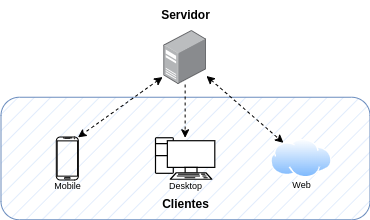
\includegraphics[width=0.5\textwidth]{media/content/estado-arte/client-server.png}
    \caption{Arquitetura Cliente-Servidor}
    \label{fig:client-server}
\end{figure}

\subsection{Arquitetura Streaming}

Os sistemas de \textit{streaming} distribuídos são cruciais para o processamento e a análise de dados 
em tempo real. O desempenho destes sistemas depende, em grande parte, da distribuição efetiva da 
carga de trabalho entre as máquinas \cite{stream2020}. Para garantir um serviço de \textit{streaming} 
eficaz e confiável, é essencial estabelecer um ambiente distribuído para o fluxo contínuo de 
informação \cite{stream2014}. A computação de \textit{streams} surgiu como uma tecnologia líder 
para analisar e gerir dados de fluxo massivo, tornando-se um modelo popular para a análise de 
fluxo de dados em tempo real \cite{stream2018} \cite{stream2018b}.

O \textit{Apache Storm}, um sistema de \textit{streaming} distribuído, foi reconhecido como um 
sistema de processamento de \textit{streams} de dados distribuídos tolerante a falhas em tempo real, 
enfatizando a importância da tolerância a falhas no processamento de \textit{streams} 
\cite{stormattwitter}. Num sistema de processamento distribuído de \textit{streams}, estes dados 
são processados em tempo real por um conjunto de operadores distribuídos por um \textit{cluster} de 
servidores, o que demonstra a natureza distribuída dos sistemas de processamento do fluxos de dados.

\subsection{Problemas de consenso}

O problema do consenso em sistemas de \textit{software} distribuídos é uma questão fundamental que 
tem merecido grande atenção nos últimos anos devido à sua vasta aplicação em vários domínios, como
as redes de sensores, o controlo cooperativo de sistemas multiagente e as redes inteligentes 
distribuídas \cite{consensus2020}. O consenso refere-se ao processo de desenvolvimento de políticas 
de controlo distribuído que permitem que um grupo de agentes seja capaz de chegar a um acordo sobre 
um determinado assunto \cite{consensus2013}. É uma questão crítica em algoritmos distribuídos e é
essencial para o funcionamento fiável de sistemas distribuídos assíncronos \cite{consesus2016} 
\cite{consensus2011}.

Além disso, o problema do consenso foi investigado no contexto de restrições e condições
específicas, como restrições de entrada e latência na comunicação, levando ao desenvolvimento de
algoritmos como o algoritmo de consenso projetado e o algoritmo de subgradiente para estimativa 
de consenso em sistemas multiagentes com restrições convexas e atrasos de comunicação 
\cite{consensus2018}.

\section{Estratégias de implantação}

Esta secção explora algumas das abordagens de implantação e atualização de aplicações, com foco 
especial em algumas técnicas em específico como \textit{canary deployment} e \textit{rolling update}.
Ao examinar várias estratégias em detalhe, podemos capturar a essência das práticas de implantação, 
identificando os seus benefícios, desafios e áreas de aplicação mais adequadas. 

\subsection{Canary Deployment}

A técnica de \textit{canary deployment} é uma estratégia de implantação de \textit{software} que 
tem ganhado atenção na literatura nos últimos tempos. Esta técnica é brevemente introduzida no 
contexto da implantação contínua de produtos e serviços com uso intensivo de \textit{software} \cite{canary2017}. 
A estratégia de implantação \textit{canary} envolve lançar uma parte das atualizações do sistema a 
um subconjunto de utilizadores, permitindo detetar problemas antes da implantação completa.
Este processo pode ser ilustrado na Figura \ref{fig:canary-before} e na Figura \ref{fig:canary-after}. 
Esta estratégia permite uma implementação gradual e segura das alterações, minimizando o impacto 
para a maior parte do utilizadores em caso de falha. Esta estratégia é proposta para uma implantação 
bem sucedida no contexto de estratégias híbridas de implantação de \textit{software} para sistemas 
complexos \cite{canary2022}. É também importante destacar a importância das \textit{pipelines} 
automatizadas de implantação no contexto de \ac{CI} e \ac{CD}, onde o sucesso da adoção das 
alterações nas empresas depende fortemente das \textit{pipelines} de implantação 
\cite{canary2017b}. Além disso, foi proposta a utilização da implantação \textit{canary} como um 
padrão de implantação de \textit{software} para controlar a implantação de novas versões de 
\textit{software}, diminuindo o risco de falhas no processo e aumentando a confiabilidade 
\cite{canary2021}.

\begin{figure}[H]
    \centering
    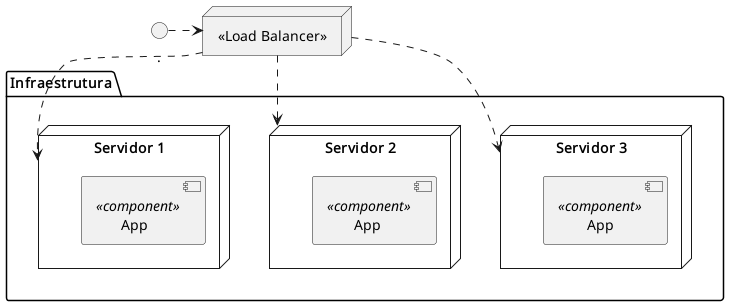
\includegraphics[width=0.4\textwidth]{media/content/estado-arte/canary-before.png}
    \caption{Estratégia de implantação \textit{canary} antes da atualização}
    \label{fig:canary-before}
\end{figure}

\begin{figure}[H]
    \centering
    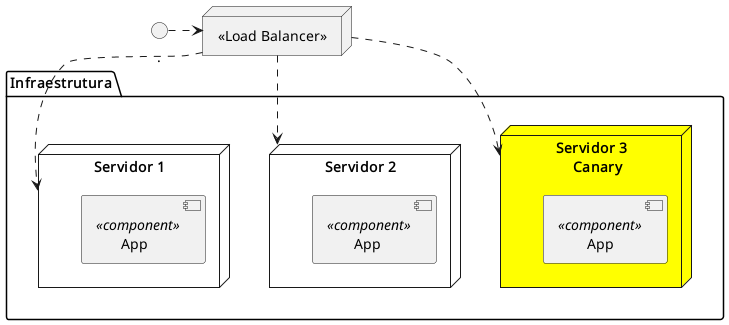
\includegraphics[width=0.4\textwidth]{media/content/estado-arte/canary-after.png}
    \caption{Estratégia de implantação \textit{canary} após a atualização}
    \label{fig:canary-after}
\end{figure}

\subsection{Rolling Update}

A estratégia de implementação de \textit{rolling update}, ou atualizações contínuas, é um aspeto 
crucial da manutenção e gestão de \textit{software}, em particular no contexto da computação em 
\textit{cloud} \cite{rolling2014}. Esta estratégia envolve atualizar gradualmente as instâncias de 
um serviço, substituindo cada instância antiga por uma nova, de forma sequencial, garantindo assim 
a disponibilidade contínua do serviço durante o processo de atualização. Nesta estratégia é destacada 
a importância da atualização contínua como uma técnica para a atualização dinâmica de \textit{software} 
que se encontra a ser utilizado ativamente por clientes \cite{rolling2014}. 

Neste tipo de abordagens é importante ter em conta a engenharia de tráfego e a necessidade de 
introduzir nós de reserva e de sentinela nas redes do sistema \cite{canary2022}, salientando a 
relevância da implementação de versões \textit{canary} como base para a estratégia de atualização 
do cliente \cite{canary2022}. A presença deste tipo de nós na rede neste tipo de estratégia é 
crucial para garantir a disponibilidade contínua do serviço durante o processo de atualização e a 
deteção de problemas antes da implantação completa.

\subsection{Blue-Green Deployment}

A implantação \textit{blue-green} é uma estratégia de implantação de \textit{software} que visa 
minimizar o tempo de indisponibilidade e os riscos associados às atualizações de \textit{software}, 
garantindo a disponibilidade e confiabilidade contínua do sistema. Esta estratégia envolve a
manutenção de dois ambientes de produção idênticos, Figura \ref{fig:blue-green-before} - o ambiente atual 
(\textit{blue}) e o novo (\textit{green}), e o encaminhamento do tráfego de utilizadores entre eles. 
Quando se pretende implantar uma nova versão do sistema, o tráfego é gradualmente transferido do 
ambiente "azul" para o ambiente "verde" como ilustrado na Figura \ref{fig:blue-green-after}, 
permitindo atualizações sem indisponibilidade e simplificando o processo de reversão das 
alterações, se necessário \cite{canary2022}.

A abordagem híbrida da implantação de software, combina a implantação \textit{canary} e a técnica 
\textit{blue-green} com a abordagem de lançamento \textit{dark} - um ambiente de intermédio, semelhante
ao de produção, que opera com dados reais - e o uso de \textit{flags} de funcionalidades, 
melhorando a estratégia global de implantação \cite{canary2022}. Esta abordagem assegura uma 
transição suave entre versões e permite a realização de testes num ambiente semelhante ao de 
produção antes da implantação para a totalidade dos utilizadores.

A técnica de implantação \textit{blue-green} baseada em descoberta de serviço em ambientes de 
\textit{cloud}, é enfatizada em ambientes modernos de computação distribuída \cite{bluegreen}. 
Desta forma, podemos concluir a importância da implantação \textit{blue-green} em sistemas baseados 
em \textit{cloud}, onde a alta disponibilidade e a interrupção mínima são cruciais.

\begin{figure}[H]
    \centering
    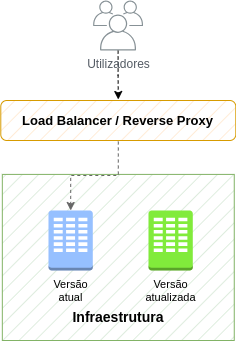
\includegraphics[width=0.3\textwidth]{media/content/estado-arte/blue-green-before.png}
    \caption{Estratégia de implantação \textit{blue-green} antes da atualização}
    \label{fig:blue-green-before}
\end{figure}

\begin{figure}[H]
    \centering
    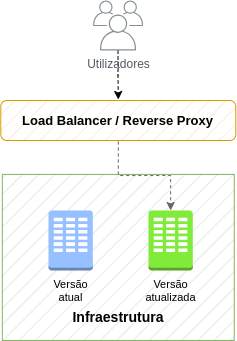
\includegraphics[width=0.3\textwidth]{media/content/estado-arte/blue-green-after.png}
    \caption{Estratégia de implantação \textit{blue-green} após a atualização}
    \label{fig:blue-green-after}
\end{figure}

\section{Monitorização de Sistemas}

A monitorização de sistemas de \textit{software} é uma prática essencial para garantir a saúde, 
desempenho e segurança de aplicações. Esta atividade envolve a obtenção e análise contínua de métricas, 
registos de eventos, \textit{logs} e outros dados relevantes, para avaliar o estado e o comportamento 
do sistema. Estas informações permitem tirar conclusões importantes sobre o desempenho da aplicação, 
ajudando as equipas de operações a detetar problemas, identificar tendências de comportamento, 
otimizar recursos e responder proativamente a eventos, contribuindo assim para a manutenção de 
operações eficazes.

\subsection{Métricas}

As métricas de monitorização são essenciais em projetos de \textit{software}, permitindo a descrição 
quantitativa dos projetos e a avaliação de métodos e ferramentas para aumentar a produtividade e a 
qualidade das soluções \cite{metrics2003}. Este tipo de monitorização é crucial para controlar 
projetos, produtos e processos de \textit{software} \cite{metrics2019}. As métricas permitem que os 
gestores de projetos e desenvolvedores acompanhem, e controlem, os projetos em que estão a trabalhar,
fornecendo informações sobre o estado e o progresso da solução \cite{metrics2016}. As 
métricas ajudam a estimar e a prever projectos futuros, incluindo riscos e custos 
\cite{metrics2016b}. A utilização de métricas é vital para determinar as características de 
qualidade do \textit{software} e avaliar a saúde de um projeto \cite{metrics2015}.

O \textit{Grafana} \cite{grafana}, juntamente com outras ferramentas como o \textit{Elastic Search}
\cite{elastic-search} é amplamente utilizado para visualizar dados de séries temporais e monitorizar
a evolução de questões de dívida técnica em projetos de \textit{software} \cite{metrics2019b}. O 
\textit{Grafana} é também utilizado para obter, armazenar e visualizar metadados produzidos por 
sistemas de gestão de dados e fluxo de trabalho, demonstrando a sua importância na monitorização 
de projetos \cite{metrics2021}. O \textit{Grafana} serve como uma ferramenta de visualização para 
processar pontos de dados brutos e interfaces de monitorização, destacando sua versatilidade na 
monitorização de projetos de \textit{software} \cite{metrics2022}.

\subsection{Registo de eventos}

O registo de eventos desempenha um papel crucial na engenharia de \textit{software} uma vez que 
fornece uma noção das atividades e dos eventos que ocorrem no sistema \cite{logs2022}. A profundidade 
do conhecimento disponível nos \textit{logs} levou ao desenvolvimento de plataformas comerciais de 
análise deste tipo de eventos, como o \textit{Splunk} \cite{splunk}, que são essenciais para 
analisar e compreender os dados de \textit{logs} \cite{logs2021}. No entanto, existem desafios nos 
registos de eventos durante o desenvolvimento de projetos de \textit{software}, particularmente em 
projetos \textit{open source}, o que leva a uma redução na rastreabilidade dos defeitos e à
deteção de \textit{bugs} de \textit{software} \cite{logs2018}. Os \textit{logs} servem diferentes 
propósitos, como deteção de anomalias, diagnóstico de problemas, verificação de programas, análise 
de uso e monitorização  de segurança, destacando assim a sua importância em sistemas de
\textit{software} robustos e seguros \cite{logs2019}.


\oddPageStart
\chapter{Análise e Desenho da Solução}
\label{sec:3-Analise}

Depois de contextualizados os temas relevantes, o presente capítulo foca-se na análise do problema 
que sustenta este relatório e na apresentação do desenho da solução criada.

\section{Domínio do Problema}

O fluxo que trata da informação de catálogo é dos mais sensíveis e cruciais para o bom funcionamento
dos sistemas que integram os serviços do grupo Flutter. Este fluxo funciona em tempo-real recorrendo
ao uso de \textit{streams} para conseguir atingir este objetivo. Esta abordagem permite garantir
o processamento assíncrono dos dados relativos a este fluxo de uma forma otimizada.

De momento, os serviços responsáveis pelo processamento destes dados estão distribuídos em dois
\glspl{cluster} que usam \textit{Apache Storm} para a gestão do mesmo. Esta solução apresenta algumas
limitações passíveis de análise por forma a melhorar a capacidade de escalabilidade destes serviços. 

A primeira destas limitações é o elevado número de \ac{VM} presente em cada \gls{cluster}. Este 
problema impacta a solução na fase de lançamento de novas versões. Isto deve-se ao facto de toda a 
infraestrutura estar sob demanda constante com vários lançamentos paralelos de vários serviços em 
ao ser necessário criar novas \ac{VM} o processo responsável pela gestão de máquinas da
infraestrutura pode não ser capaz de responder ao pedido. Desta forma, diminuir o número de \ac{VM}
presentes no \gls{cluster} representaria uma melhoria na probabilidade da taxa de sucesso de
lançamento de uma nova versão (em todos os ambientes).

Além disso, existem topologias presentes em certos \glspl{cluster} que estão a usar um excesso de
recursos face aos recursos que necessitam para operar sem falhas em alturas de pico de utilização
dos mesmos.

\subsection{Contexto}

O grupo Flutter é uma das maiores empresas de apostas desportivas a nível mundial. Este grupo
possui várias marcas que operam em diferentes mercados, como o mercado britânico, australiano e
norte-americano. A empresa tem vindo a crescer de forma exponencial nos últimos anos e, como tal,
tem vindo a investir em novas tecnologias e a expandir a sua presença em novos mercados. No mercado
de \ac{UKI} o grupo Flutter adquiriu, nos últimos meses uma nova marca - \ac{SBG} \cite{skybet}. 
Esta aquisição requer que os serviços necessários para a operação da marca dentro da infraestrutura 
do grupo seja migrada para a mesma. De momento, o \textit{hardware} disponível nos \glspl{dc} da 
empresa não é capaz de suprir as necessidades de processamento necessária para hospedar estes 
serviços, logo, é necessário levar a cabo um processo de otimização de recursos nos \glspl{cluster} 
existentes de forma a tornar possível que o serviço opere sem falhas.

\subsection{Modelo de Domínio}

Nesta secção vai ser apresentado o \ac{MD} simplificado do fluxo de catálogo disponibilizado nas 
plataformas de \textit{sportsbook} das empresas do grupo Flutter. A compreensão deste modelo será
importante para acompanhar a solução apresentada de seguida. A Figura \ref{md} apresenta a vista
simplificada deste modelo.

\begin{figure}[H]
  \centerline{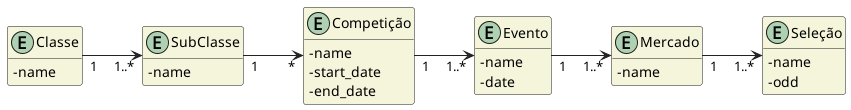
\includegraphics[scale=0.4]{media/content/analise/dm.png}}
  \caption{Modelo de Domínio - Fluxo de Catálogo (simplificado)}
  \label{md}
\end{figure}

De forma a ser mais simples acompanhar os termos apresentados na Figura \ref{md} vamos proceder 
a descrever uma hierarquia de exemplo:

\begin{itemize}
  \item \textbf{Classe} - Desporto (exemplo: Futebol)
  \item \textbf{SubClasse} - Especificação de Desporto (exemplo: Futebol Masculino)
  \item \textbf{Competição} - Competição (exemplo: Liga Portuguesa de Futebol)
  \item \textbf{Evento} - Evento (exemplo: FC Porto vs SC Espinho)
  \item \textbf{Mercado} - Tipo de Aposta (exemplo: Resultado Final)
  \item \textbf{Seleção} - Seleção de Aposta (exemplo: SC Espinho a vencer)
\end{itemize}

Como referido anteriormente, esta representação é apenas uma simplificação da realidade, isto
porque cada classe pode ter diferenças significativas na forma como representa a restante
hierarquia de relações entre entidades.

\section{Engenharia de Requisitos}

A Engenharia de Requisitos é uma área muito relevante no desenvolvimento de \textit{software}, pois 
sustenta a análise dos projetos, a primeira fase em que a equipa de desenvolvimento consegue 
compreender o domínio do negócio para o qual estão a desenvolver uma solução. Este passo representa 
o processo de obtenção de requisitos através de uma análise do problema e pressupõe a definição 
das necessidades, tanto por parte do cliente, como por necessidades técnicas, na procura de uma 
solução clara que valide a proposta apresentada. Seguindo um processo estruturado e adotando as 
melhores práticas, passamos a promover uma melhor comunicação entre as várias partes interessadas.

Considerando os aspetos mencionados, nesta secção serão apresentados os requisitos do sistema 
identificados e requisitados no início do projeto de maneira a garantir a que a solução desenvolvida 
vai de encontro com as necessidades apresentadas inicialmente. Estes requisitos podem ser 
categorizados em funcionais - funcionalidades distintas e essenciais que o sistema deve realizar, 
e não funcionais - restrições impostas para que o sistema realize os requisitos funcionais 
corretamente.

\subsection{Requisitos Não Funcionais}

Os requisitos não funcionais não se concentram no que o sistema faz, mas sim em como é esperado que
ele funcione. 

Os requisitos não funcionais apresentados de seguida, guiam-se pelo modelo FURPS+, um padrão de 
classificação qualitativa das características de um \textit{software} (\textbf{F}unctionality, 
\textbf{U}sability, \textbf{R}eliability, \textbf{P}erformance, \textbf{S}upportability), para 
facilitar a compreensão dos mesmos. O "\textbf{+}" refere-se a métodos de classificação diferentes, 
como por exemplo, restrições de design, implementação, interface ou físicos.

Estes requisitos são mais complexos de definir a nível do \gls{cluster}, pois cada topologia tem 
uma finalidade diferente, pelo que os requisitos são ligeiramente diferentes entre eles. De uma
forma geral, o sistema deve:

Para estes requisitos são definidos, para cada topologia, \acp{SLI} - os indicadores que mostram o
desempenho do sistema a todo o momento, \acp{SLO} - os objetivos que a equipa de desenvolvimento
deve atingir de forma a cumprir os \acp{SLA} - o acordo que o sistema mantém com os clientes a 
nível do seu funcionamento.

\vspace{5mm}

\textbf{Funcionalidade}
\begin{itemize}
  \item Encontram-se especificados na subsecção \nameref{sec:3-rf}.
\end{itemize}

\textbf{Usabilidade}
\begin{itemize}
  \item Não aplicável.
\end{itemize}

\textbf{Fiabilidade}

\begin{itemize}
  \item O sistema deve ser capaz de recuperar de falhas de funcionamento sem perda de dados.
  \item O sistema deve ser capaz de recuperar de falhas de funcionamento minimizando o tempo de inatividade.
  \item O sistema deve ser capaz de recuperar de falhas de funcionamento sem intervenção manual.
\end{itemize}

\textbf{Desempenho}
\begin{itemize}
  \item O sistema deve manter a capacidade de processamento que tinha antes da intervenção.
  \item O sistema deve ser capaz de processar transações em dia de pico de catálogo \footnote[1]{
    Os "dias de pico de catálogo" são dias identificados previamente em que são criados muitos 
    eventos novos ou dias em que estão a ser realizados muitos eventos em simultâneo}
    sem atrasos significativos na latência.
  \item O sistema deve ser capaz de processar transações em dia de pico de catálogo \footnotemark[1] minimizando o 
    tempo de resposta.
\end{itemize}

\textbf{Suporte}
\begin{itemize}
  \item O sistema deve ter, pelo menos, 80\% de cobertura de testes.
  \item O sistema deve suportar a replicação de \glspl{cluster} em dois \glspl{dc}.
  \item O sistema deve suportar a configuração de quatro ambientes - \ac{QA}, desenvolvimento, 
    performance e produção.
  \item O sistema deve ter suporte 24/7 com uma equipa de \gls{on-call} disponível.
\end{itemize}

\textbf{Restrições de Design}
\begin{itemize}
  \item O sistema deve suportar quatro ambientes - \ac{QA}, desenvolvimento, 
    performance e produção.
  \item O sistema deve estar replicado em dois \glspl{dc}.
  \item Todas as \ac{VM} do mesmo \gls{cluster} devem ter o mesmo \gls{flavour}.
  \item A paralelização deve ser feita por \ac{VM} e não por processo. Ou seja, a mesma \ac{VM} 
    não pode ter dois processos a correr em paralelo.
\end{itemize}

\subsection{Requisitos Funcionais}
\label{sec:3-rf}

Os requisitos funcionais especificam as unidades funcionais de um sistema de \textit{software}.
Estes requisitos concentram-se nas funções que devem ser disponibilizadas, descrevem as
funcionalidades, comportamentos e operações específicas que os utilizadores devem ser capazes de 
executar, podendo variar desde ações básicas, como entrada e saída de dados, a algoritmos 
específicos e processos de negócio.

De forma a facilitar a compreensão dos requisitos funcionais estes encontram-se descritos na 
Tabela \ref{tab:reqfun} e na Figura \ref{dcu}, na forma de \textit{User Stories}, seguindo a 
estrutura apresentada no artigo "(User) Stories for Analytics Projects - Part 1". \cite{us}.

% \begin{table}[H]
%   \begin{center}
%     \caption{Requisitos Funcionais}
%     \vspace{5mm}
%     \label{tab:reqfun}
%     \begin{tabular}{|c|l|}
%       \hline
%       ID & User Story                                                                  \\ \hline
%       1  & \begin{tabular}[c]{@{}l@{}}Como Engenheiro de Aplicações, pretendo que seja efetuado \\
%         um estudo que determine possíveis otimizações de recursos nos \glspl{cluster} dos serviços \\
%       de catálogo .\end{tabular} \\ \hline
%       2  & \begin{tabular}[c]{@{}l@{}}Como Engenheiro de Aplicações, pretendo que seja elaborado \\
%         um plano que defina como serão efetuadas as alterações nos recursos dos \glspl{cluster} \\
%         dos serviços de catálogo .\end{tabular} \\ \hline
%       3  & \begin{tabular}[c]{@{}l@{}}Como Engenheiro de Aplicações, pretendo que sejam efetuadas \\
%       reduções de recursos nos \glspl{cluster} dos serviços de catálogo atuais.\end{tabular} \\ \hline
%       4  & \begin{tabular}[c]{@{}l@{}}Como Engenheiro de Aplicações, pretendo que a versão de \\
%         \textit{Apache Storm} utilizada pelos \glspl{cluster} dos serviços de catálogo seja atualizada \\
%         para a versão mais recente.\end{tabular} \\ \hline
%       5  & \begin{tabular}[c]{@{}l@{}}Como XXX, quero XXX.\end{tabular} \\ \hline
%     \end{tabular}
%   \end{center}
% \end{table}

\begin{table}[H]
  \begin{center}
    \caption{Requisitos Funcionais}
    \vspace{5mm}
    \label{tab:reqfun}
    \begin{tabular}{|c|l|}
      \hline
      ID & User Story                                                                  \\ \hline
      1  & \begin{tabular}[c]{@{}l@{}}Como utilizador, pretendo consultar os eventos ativos \\
        num determinado dia. \\
      \end{tabular} \\ \hline
        2  & \begin{tabular}[c]{@{}l@{}}Como utilizador, pretendo consultar os tipos de aposta \\
        disponíveis para um determinado evento. \\
      \end{tabular} \\ \hline
        3  & \begin{tabular}[c]{@{}l@{}}Como utilizador, pretendo consultar as \glspl{odd} de um\\
        num determinado evento. \\
      \end{tabular} \\ \hline
    \end{tabular}
  \end{center}
\end{table}

\begin{figure}[H]
  \centerline{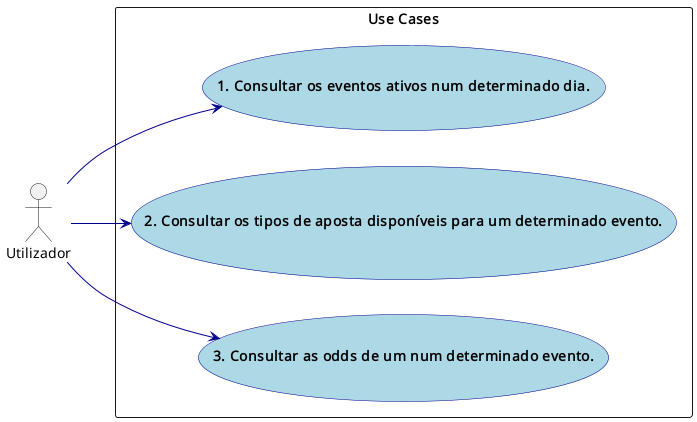
\includegraphics[scale=0.4]{media/content/analise/ucd.png}}
  \caption{Diagrama de Casos de Uso}
  \label{dcu}
\end{figure}

\section{Estado Atual do Sistema}

O sistema em análise é composto por vários \glspl{cluster} que suportam os serviços de catálogo
disponibilizados pelas marcas do grupo Flutter. Estes \glspl{cluster} são compostos por várias
\ac{VM} que executam as topologias responsáveis pelo processamento dos dados relativos a estes
serviços. A Figura \ref{strat-current} apresenta o estado atual dos \glspl{cluster}.

\begin{figure}[H]
  \centerline{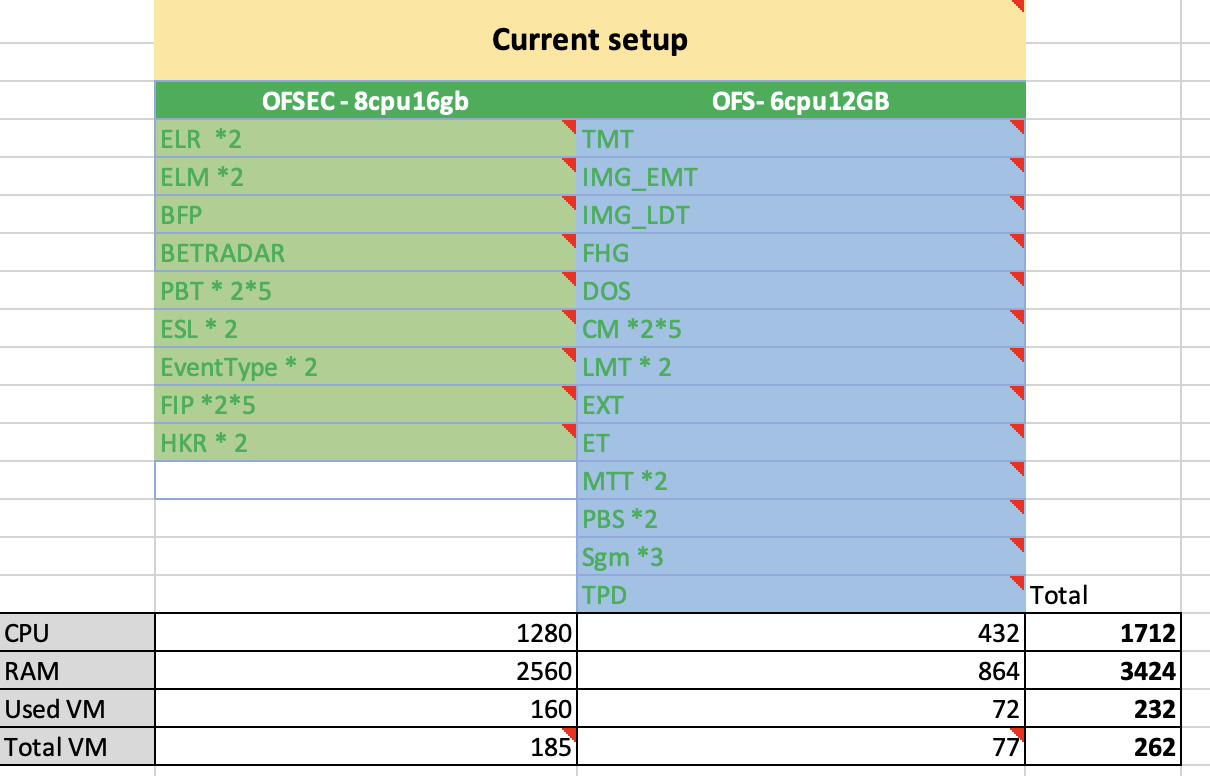
\includegraphics[scale=0.5]{media/content/analise/strat-current.png}}
  \caption{Estado atual do sistema}
  \label{strat-current}
\end{figure}

\subsection{Balanceadores de Carga}

Para lidar com falhas e garantir a disponibilidade dos serviços, os serviços de catálogo estão
distribuídos por dois \glspl{dc} e o tráfego de entrada é distribuído por um \ac{LB} que encaminha
o tráfego para os \gls{cluster} do \ac{DC} escolhido. Já a nível do \gls{cluster}, a gestão de 
tráfego e falhas é gerida pelo próprio \textit{Apache Storm} que garante a replicação dos dados
e a recuperação de falhas entre as réplicas de cada topologia.

De forma a simplificar a compreensão destes conceitos, a Figura \ref{lb} apresenta um diagrama
simplificado da arquitetura de \ac{LB} presente nos \glspl{cluster}, sendo que a gestão efetuada
a nível do \textit{Apache Storm} é simplificada como um \ac{LB} interno.

\begin{figure}[H]
  \centerline{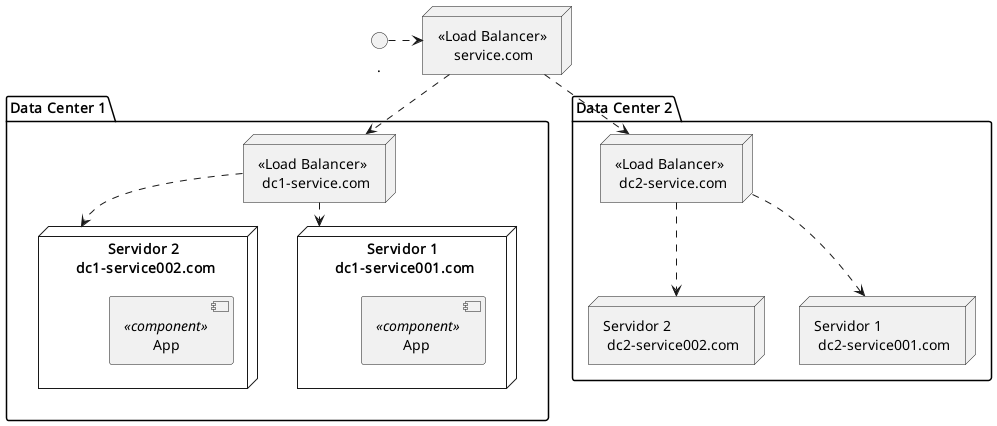
\includegraphics[scale=0.5]{media/content/analise/lb.png}}
  \caption{Arquitetura dos Balanceadores de Carga}
  \label{lb}
\end{figure}

\section{Desenho da Solução}

Após a análise do problema definido juntamente com os requisitos funcionais e não funcionais,
apresentados anteriormente, o objetivo desta secção é documentar as fases que fazem parte do
desenho da solução idealizada.

Desta forma, se for possível alterar o \gls{flavour} destes \glspl{cluster} vai ser possível economizar
recursos. Para atingir este objetivo existem várias abordagens possíveis, como por exemplo, a
alteração do número de \ac{VM} presentes em cada \gls{cluster}, a alteração do \gls{flavour}
de cada \gls{cluster} ou a alteração da distribuição de serviços por \gls{cluster}.

\subsection{Análise de Uso de Recursos}

A primeira fase do desenho da solução passa pela análise do uso de recursos dos \glspl{cluster}
que suportam os serviços de catálogo. Para tal, foram analisadas duas janelas temporais distintas
onde os serviços sofreram uma carga acima do normal. Desta forma, é possível ter uma visão clara
das possíveis otimizações de recursos a fazer já que o objetivo final é que o \gls{cluster}
mantenha a sua capacidade de processamento e seja capaz de suportar a mesma carga a que estava
sujeito antes desta intervenção.

Para isso, é importante, em primeiro lugar, compreender a forma como estes serviços são requisitados
pelo sistema para, desta forma, ser possível analisar o intervalo de datas correto. Neste caso,
todos os serviços disponibilizados pelos \glspl{cluster} são relativos ao catálogo, ou seja,
à informação relativa aos vários eventos disponibilizados aos clientes. Desta forma, os intervalos
a analisar devem ser períodos em que sejam criados muitos eventos novos, ou momentos em que
estejam a ser realizados vários eventos em simultâneo e o sistema de atualização de \glspl{odd}
esteja a ser bastante utilizado.

Após discussão com vários elementos mais experientes no negócio concluiu-se que os intervalos
adequados a esta análise seriam em agosto - quando são criados os eventos relacionados com as
principais ligas dos maiores desportos a nível europeu, como futebol e basquetebol - e dezembro 
quando existe uma nova vaga de criação de eventos nesses desportos e também a disponibilização 
dos calendários noutros desportos disponíveis nas plataformas de \textit{sportsbook} como
corridas de cavalos.

Para a análise destes dados foram usadas as métricas disponibilizadas no \textit{Grafana}. Em alguns
casos foi necessário a criação de novos \textit{dashboards} para a análise de métricas mais 
específicas para cada serviço, mas na maioria dos casos as métricas mais relevantes eram métricas 
de sistema, como uso de processador e de memória RAM.

Esta análise foca-se no uso de recursos de cada topologia. Na Figura \ref{analise-ofs} podemos
analisar o uso de recursos de um dos \glspl{cluster}. A restante análise encontra-se
presente em no Anexo \ref{appendix-a}.

\begin{figure}[H]
  \centerline{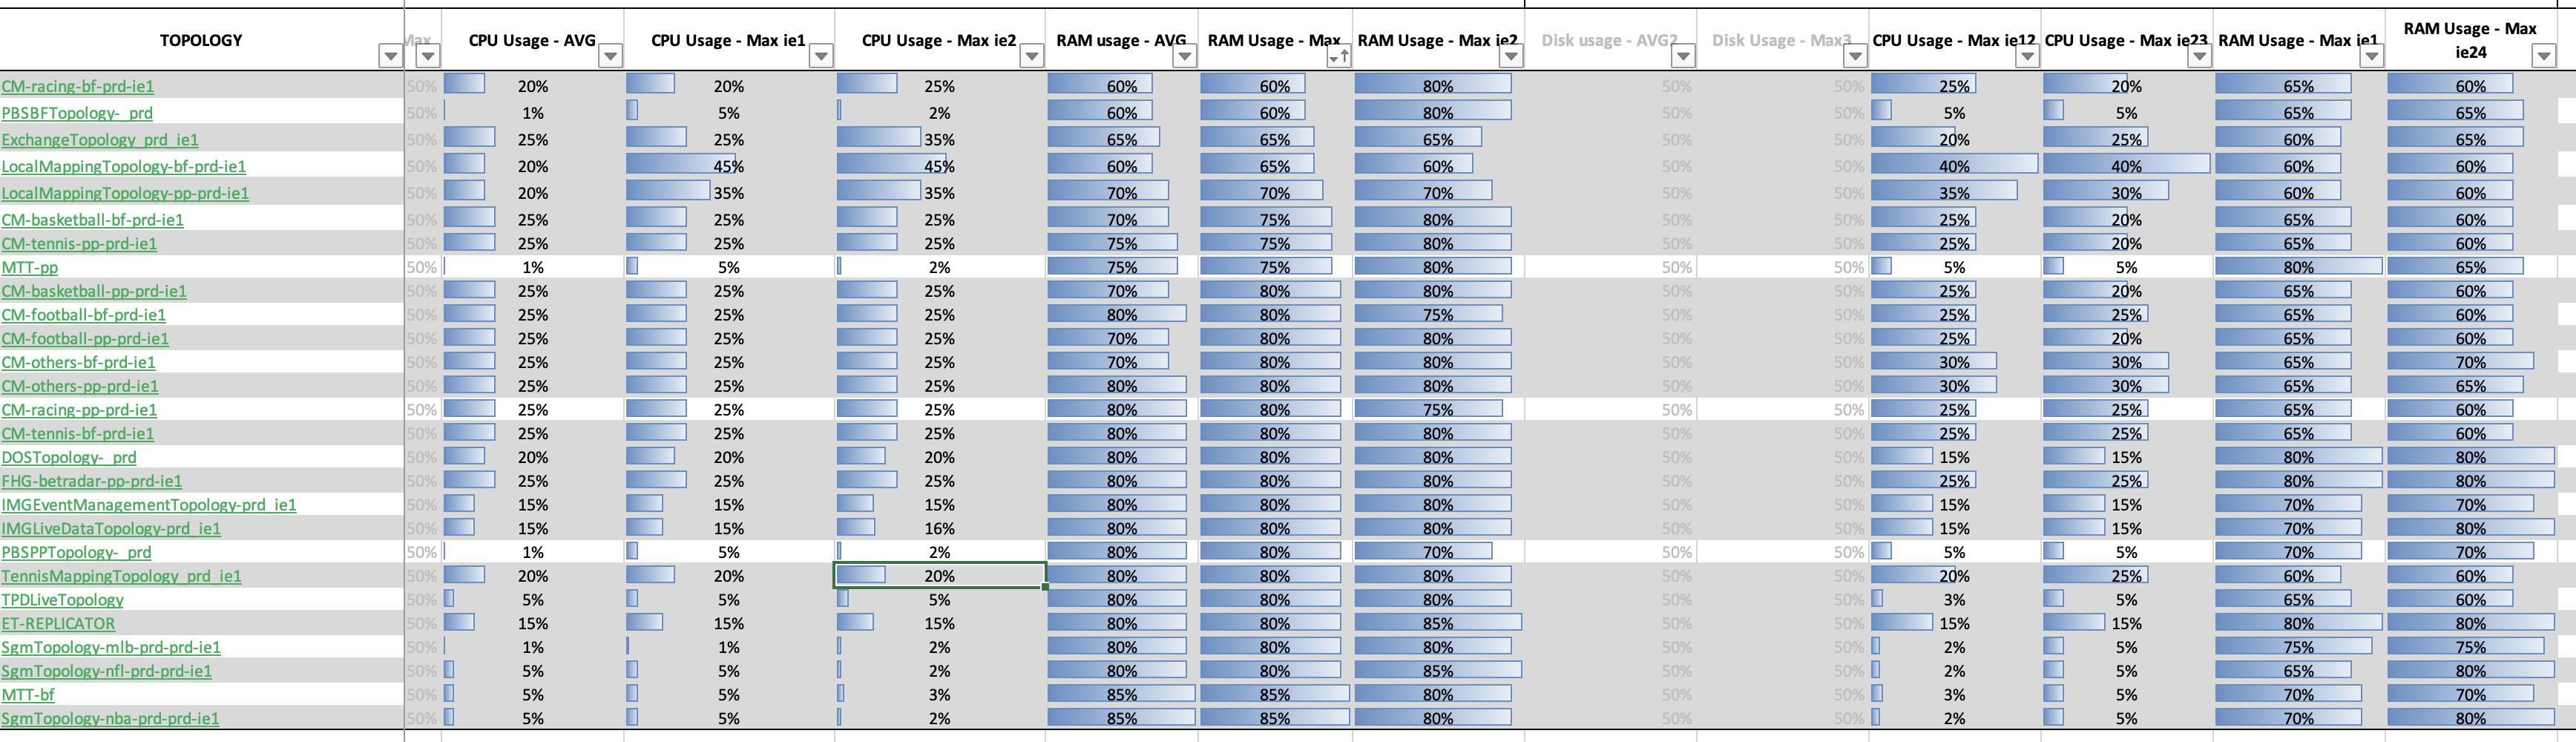
\includegraphics[scale=0.25]{media/content/analise/analise-ofs.png}}
  \caption{Análise do uso de recursos de um dos \textit{clusters}}
  \label{analise-ofs}
\end{figure}

Esta análise permitiu concluir que existem topologias que estão hospedadas num \gls{cluster}
com um \gls{flavour} superior ao que necessitam para processar a carga que lhes é atribuída,
mesmo em momentos de pico. 

\subsection{Possíveis abordagens}

Após concluída esta fase de análise foi possível sugerir novas abordagens para a distribuição
das topologias pelos \glspl{cluster} de forma a otimizar o uso total de recursos dos mesmos.

Para isso foram criadas três abordagens alternativas que tentam resolver este problema. Todas estas
abordagens vão ser analisadas e discutidas de forma a ser possível compreender qual o motivo da
escolha da alternativa que foi optada internamente.

A distribuição das topologias pelos \glspl{cluster} é apresentada, de seguida, em formato de 
tabela onde, em cada coluna é representado um \gls{cluster}, ou \ac{TLA}, como é referido 
internamente no contexto da empresa, e o respetivo \gls{flavour}. Em cada uma das células é
apresentada uma topologia e um multiplicador, por exemplo, \textit{ELR*2}. As letras são uma 
abreviatura do nome da topologia e o multiplicador refere-se à quantidade de diferentes
implementações da topologia a serem executadas no \gls{cluster}. Este multiplicador não representa
o fator de replicação da topologia, mas sim várias instâncias com implementações diferentes, por
exemplo, algumas topologias devem ter implementações diferentes por marca - topologias
\textit{brand-aware} - algumas precisam de diferentes implementações por desporto, por exemplo,
implementações diferentes para futebol e ténis.

No fim de cada tabela temos a quantidade de recursos (número de \ac{CPU} e GB de RAM) que cada 
configuração de topologias vai usar no total.

\subsubsection{Alternativa 1}

A primeira alternativa, representada na Figura \ref{proposal-1}, serve de base para todas as
alternativas que serão analisadas subsequentemente. A ideia é criar um novo \gls{cluster}
para receber as topologias que não necessitam de tanta capacidade computacional associado. Desta 
forma, será possível libertar os restantes \glspl{cluster} do número excessivo de \ac{VM} 
e, ao reduzir os \glspl{flavour} de todas as \ac{VM} procedemos à redução do uso total do
conjunto, pois é efetuada a transição de um conjunto de \ac{VM} com uma especificação, por exemplo,
4 \ac{CPU} e 12GB de memória RAM para um conjunto de \ac{VM} com 2 \ac{CPU} e 10GB RAM. No exemplo
anterior, assumindo um \gls{cluster} com 100 máquinas, teriamos uma redução de 50 \ac{CPU} e 20GB 
de RAM.

\begin{figure}[H]
  \centerline{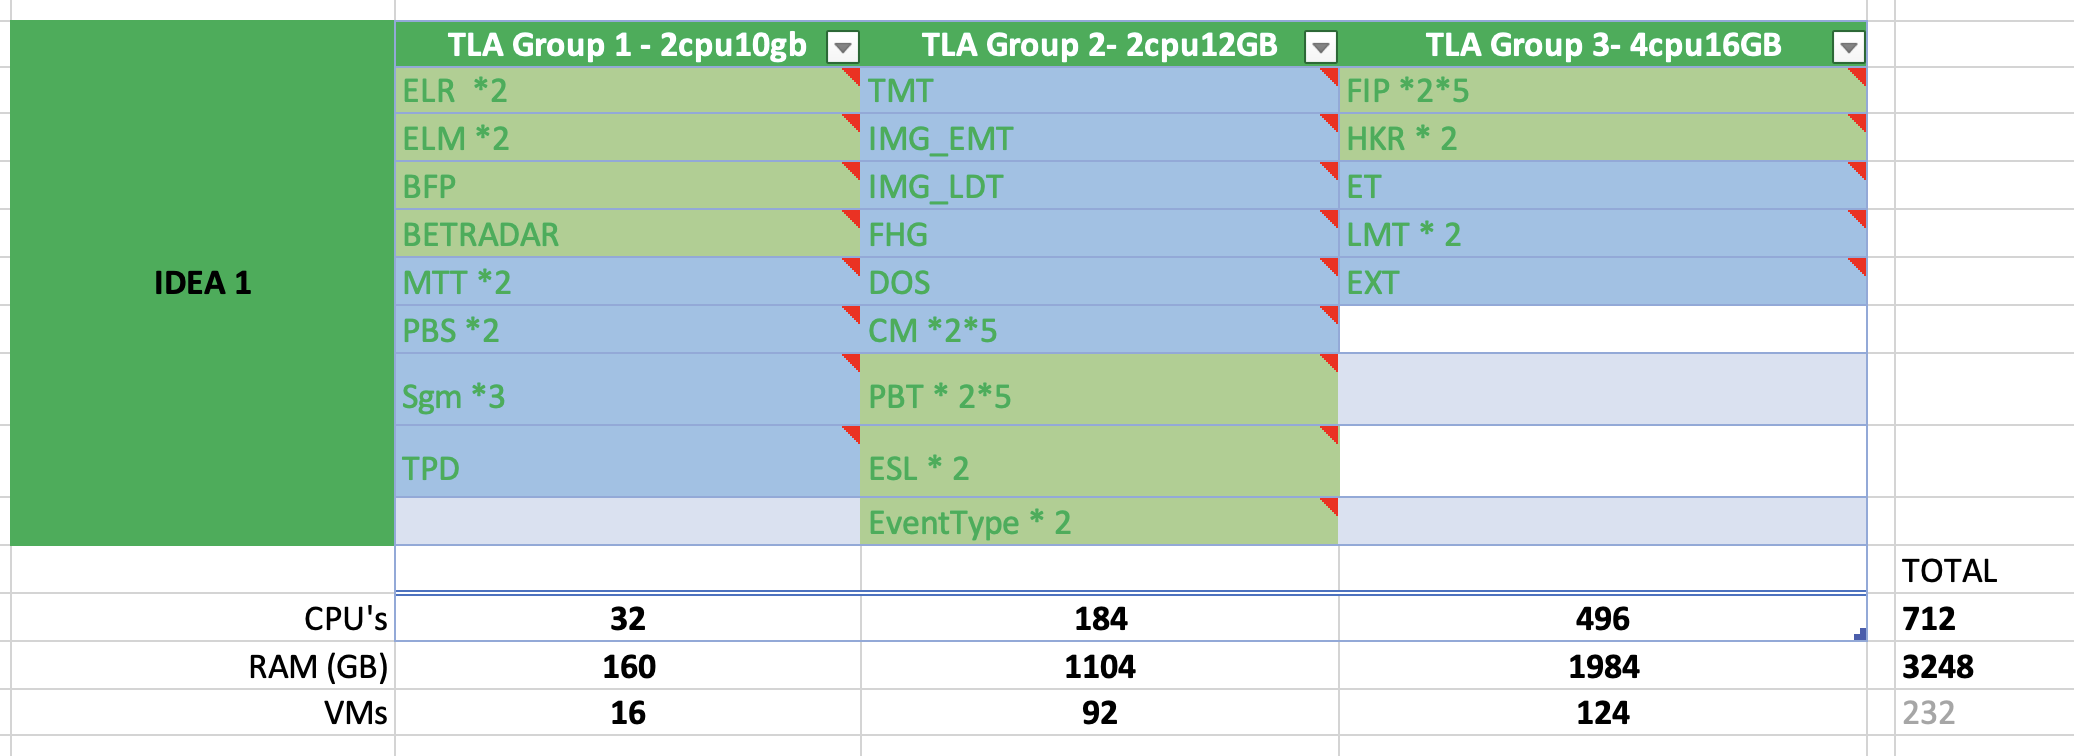
\includegraphics[scale=0.4]{media/content/analise/proposal-1.png}}
  \caption{Distribuição de topologias pelos \textit{clusters} - Alternativa 1}
  \label{proposal-1}
\end{figure}

\subsubsection{Alternativa 2}

A segunda alternativa, representada na Figura \ref{proposal-2}, diminui a memória RAM utilizada no
primeiro \gls{cluster}, além de reformular a organização das topologias pelos restantes. 

O número de \ac{VM} hospedadas no mesmo \gls{cluster} não deve ser demasiado elevado de forma a
evitar uma carga demasiado elevada no processo de implantação, isto porque, devido à forma como 
funciona o \textit{Apache Storm} a alteração numa topologia implica o processo de implantação de
todo o \gls{cluster} e, logicamente, quanto maior a quantidade de \ac{VM} que devem ser criadas
durante o processo, mais demorado se tornará.

\begin{figure}[H]
  \centerline{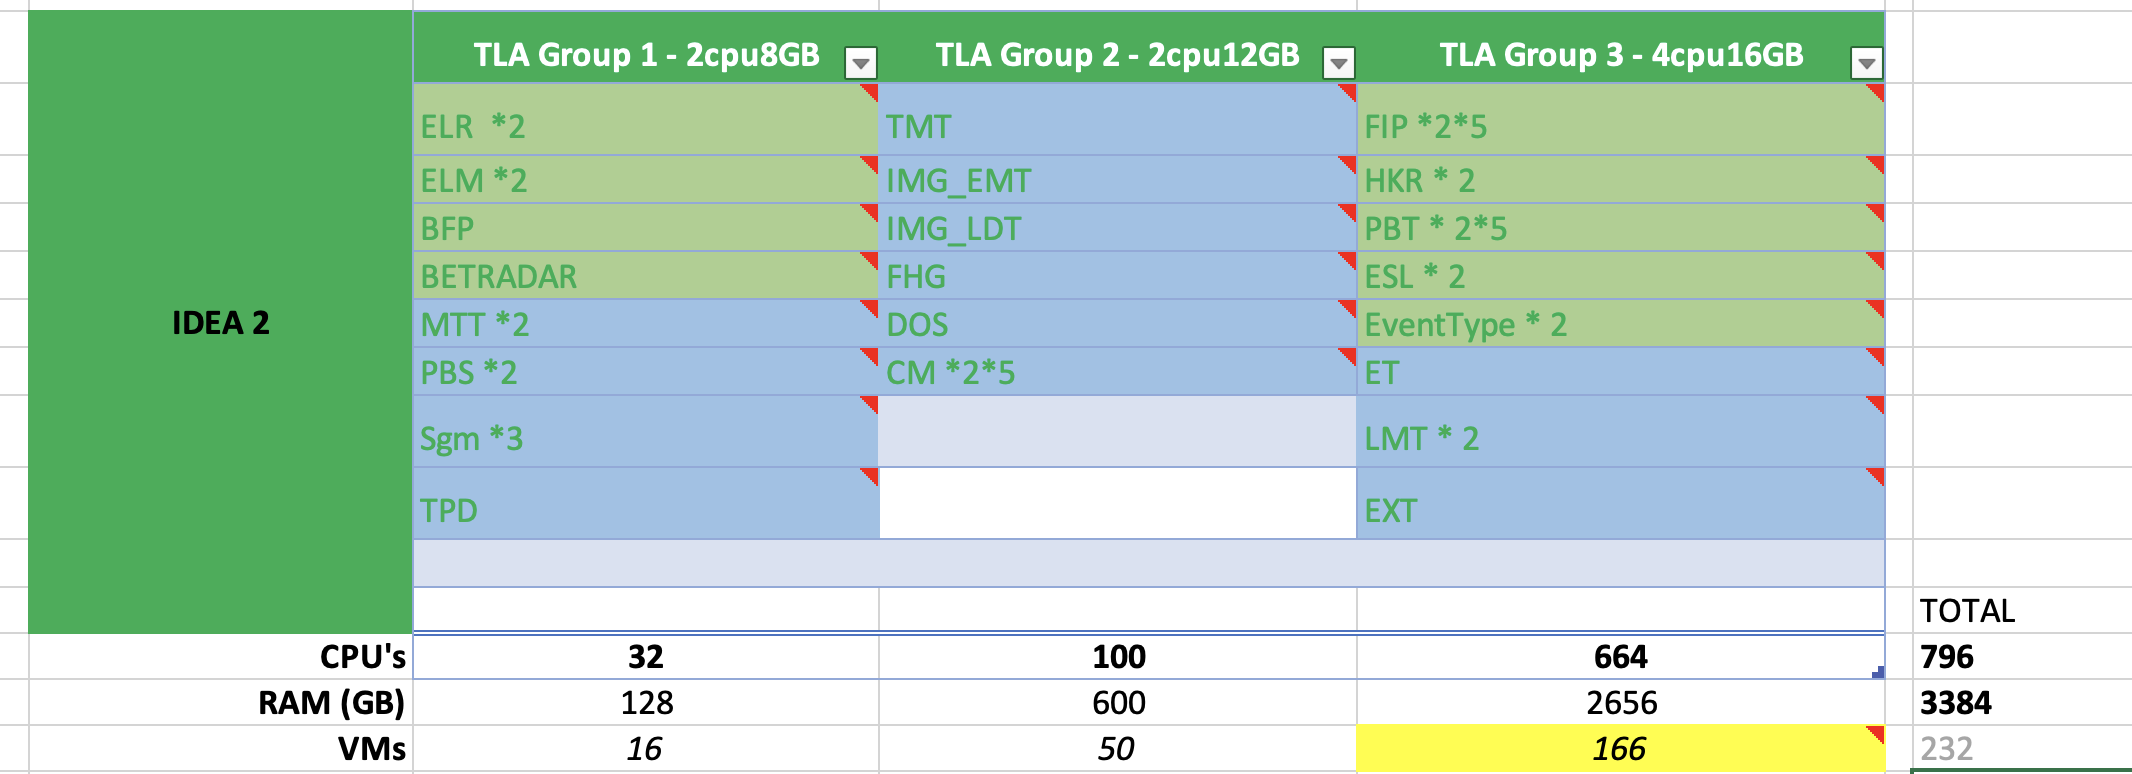
\includegraphics[scale=0.4]{media/content/analise/proposal-2.png}}
  \caption{Distribuição de topologias pelos \textit{clusters} - Alternativa 2}
  \label{proposal-2}
\end{figure}

Esta abordagem acaba por ser inferior às restantes por duas questões - o tamanho, em termos de número 
de \ac{VM}, do terceiro \gls{cluster} e a quantidade total de recursos superior à proposta
analisada anteriormente.

\subsubsection{Alternativa 3}

A terceira, e última, alternativa está representada na Figura \ref{proposal-3}.

\begin{figure}[H]
  \centerline{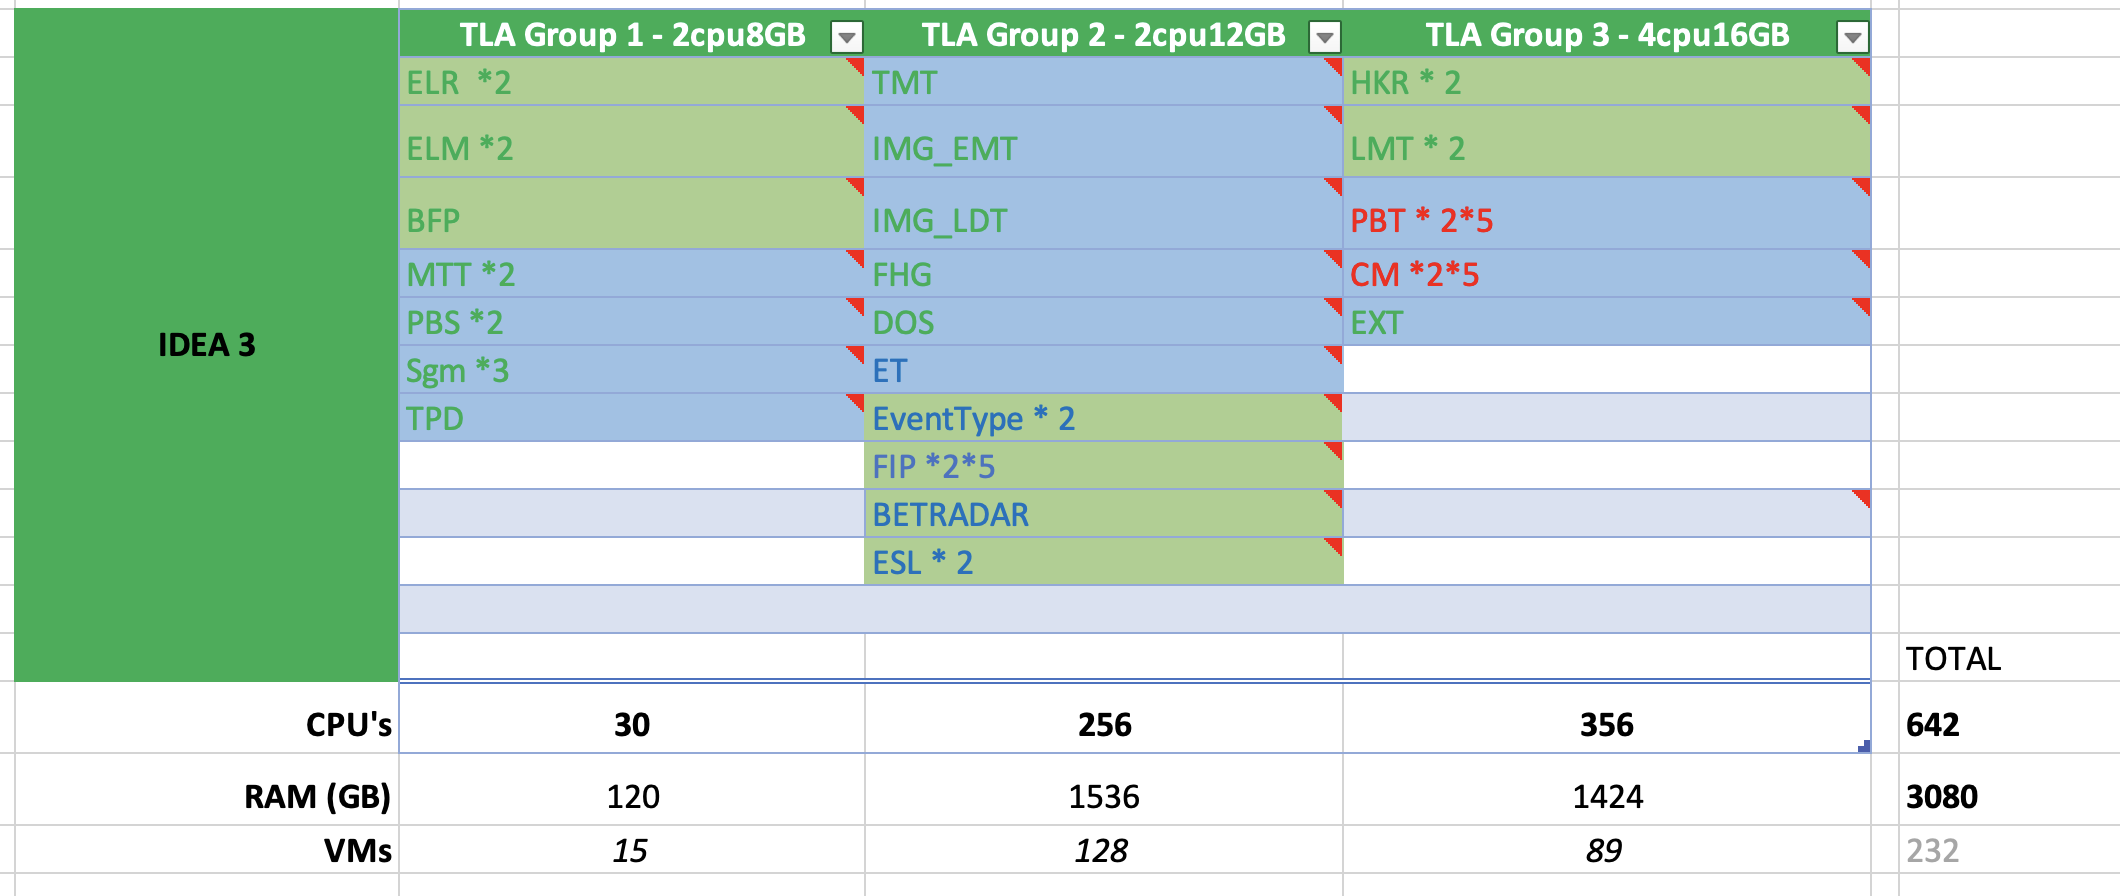
\includegraphics[scale=0.4]{media/content/analise/proposal-3.png}}
  \caption{Distribuição de topologias pelos \textit{clusters} - Alternativa 3}
  \label{proposal-3}
\end{figure}

Esta alternativa acaba por ser a mais vantajosa em quase todos os aspetos, mas acabou por ser 
descartada devido após análise por parte das equipas que desenvolvem as topologias. Isto porque uma 
das topologias é uma exceção às restantes no sentido em que todas as restantes, como mencionado 
anteriormente, na secção de \nameref{sec:3-restricao-design}, a paralelização só é permitida ser 
efetuada por máquina, ou seja, a mesma máquina não pode correr mais que um processo da topologia, 
paralelamente. Devido à necessidade acima do normal de paralelização por parte desta topologia em 
específico acabou por ser aberta a exceção e neste caso cada máquina corre dois processos em 
paralelo. Desta forma, a análise efetuada anteriormente não pode ser interpretada da mesma forma 
para esta topologia, o que invalida esta alternativa.

\subsubsection{Comparação entre alternativas}

Após uma análise cuidada de todas estas alternativas acabou por ser escolhida a primeira alternativa
com a alteração da memória RAM do primeiro \gls{cluster} chegando à opção ilustrada na Figura
\ref{proposal-final}.

\begin{figure}[H]
  \centerline{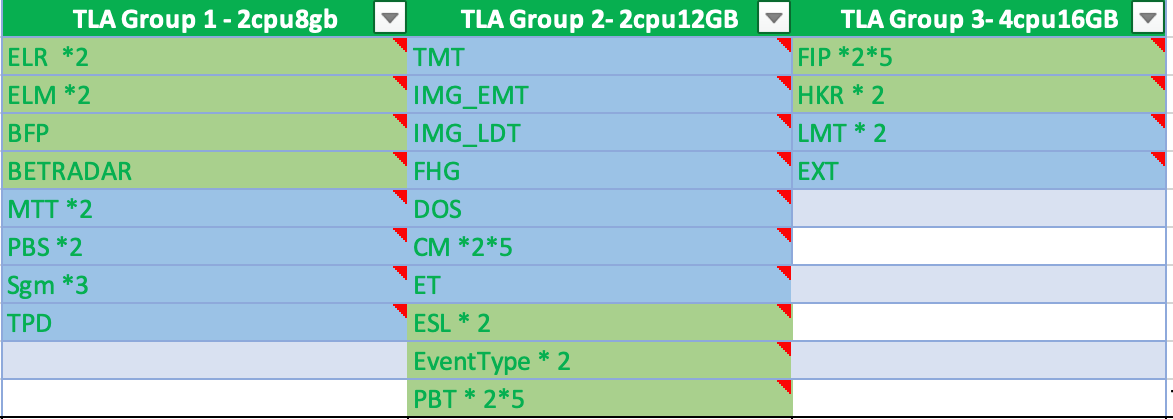
\includegraphics[scale=0.6]{media/content/analise/proposal-final.png}}
  \caption{Distribuição de topologias pelos \textit{clusters} - Alternativa Final}
  \label{proposal-final}
\end{figure}

Podemos observar na Figura \ref{comparison-proposal} a comparação entre todas as propostas
analisadas em termos de uso total de recursos em todos os ambientes, bem como a percentagem de 
redução de recursos em cada um dos parâmetros analisados (CPU e RAM).

\begin{figure}[H]
  \centerline{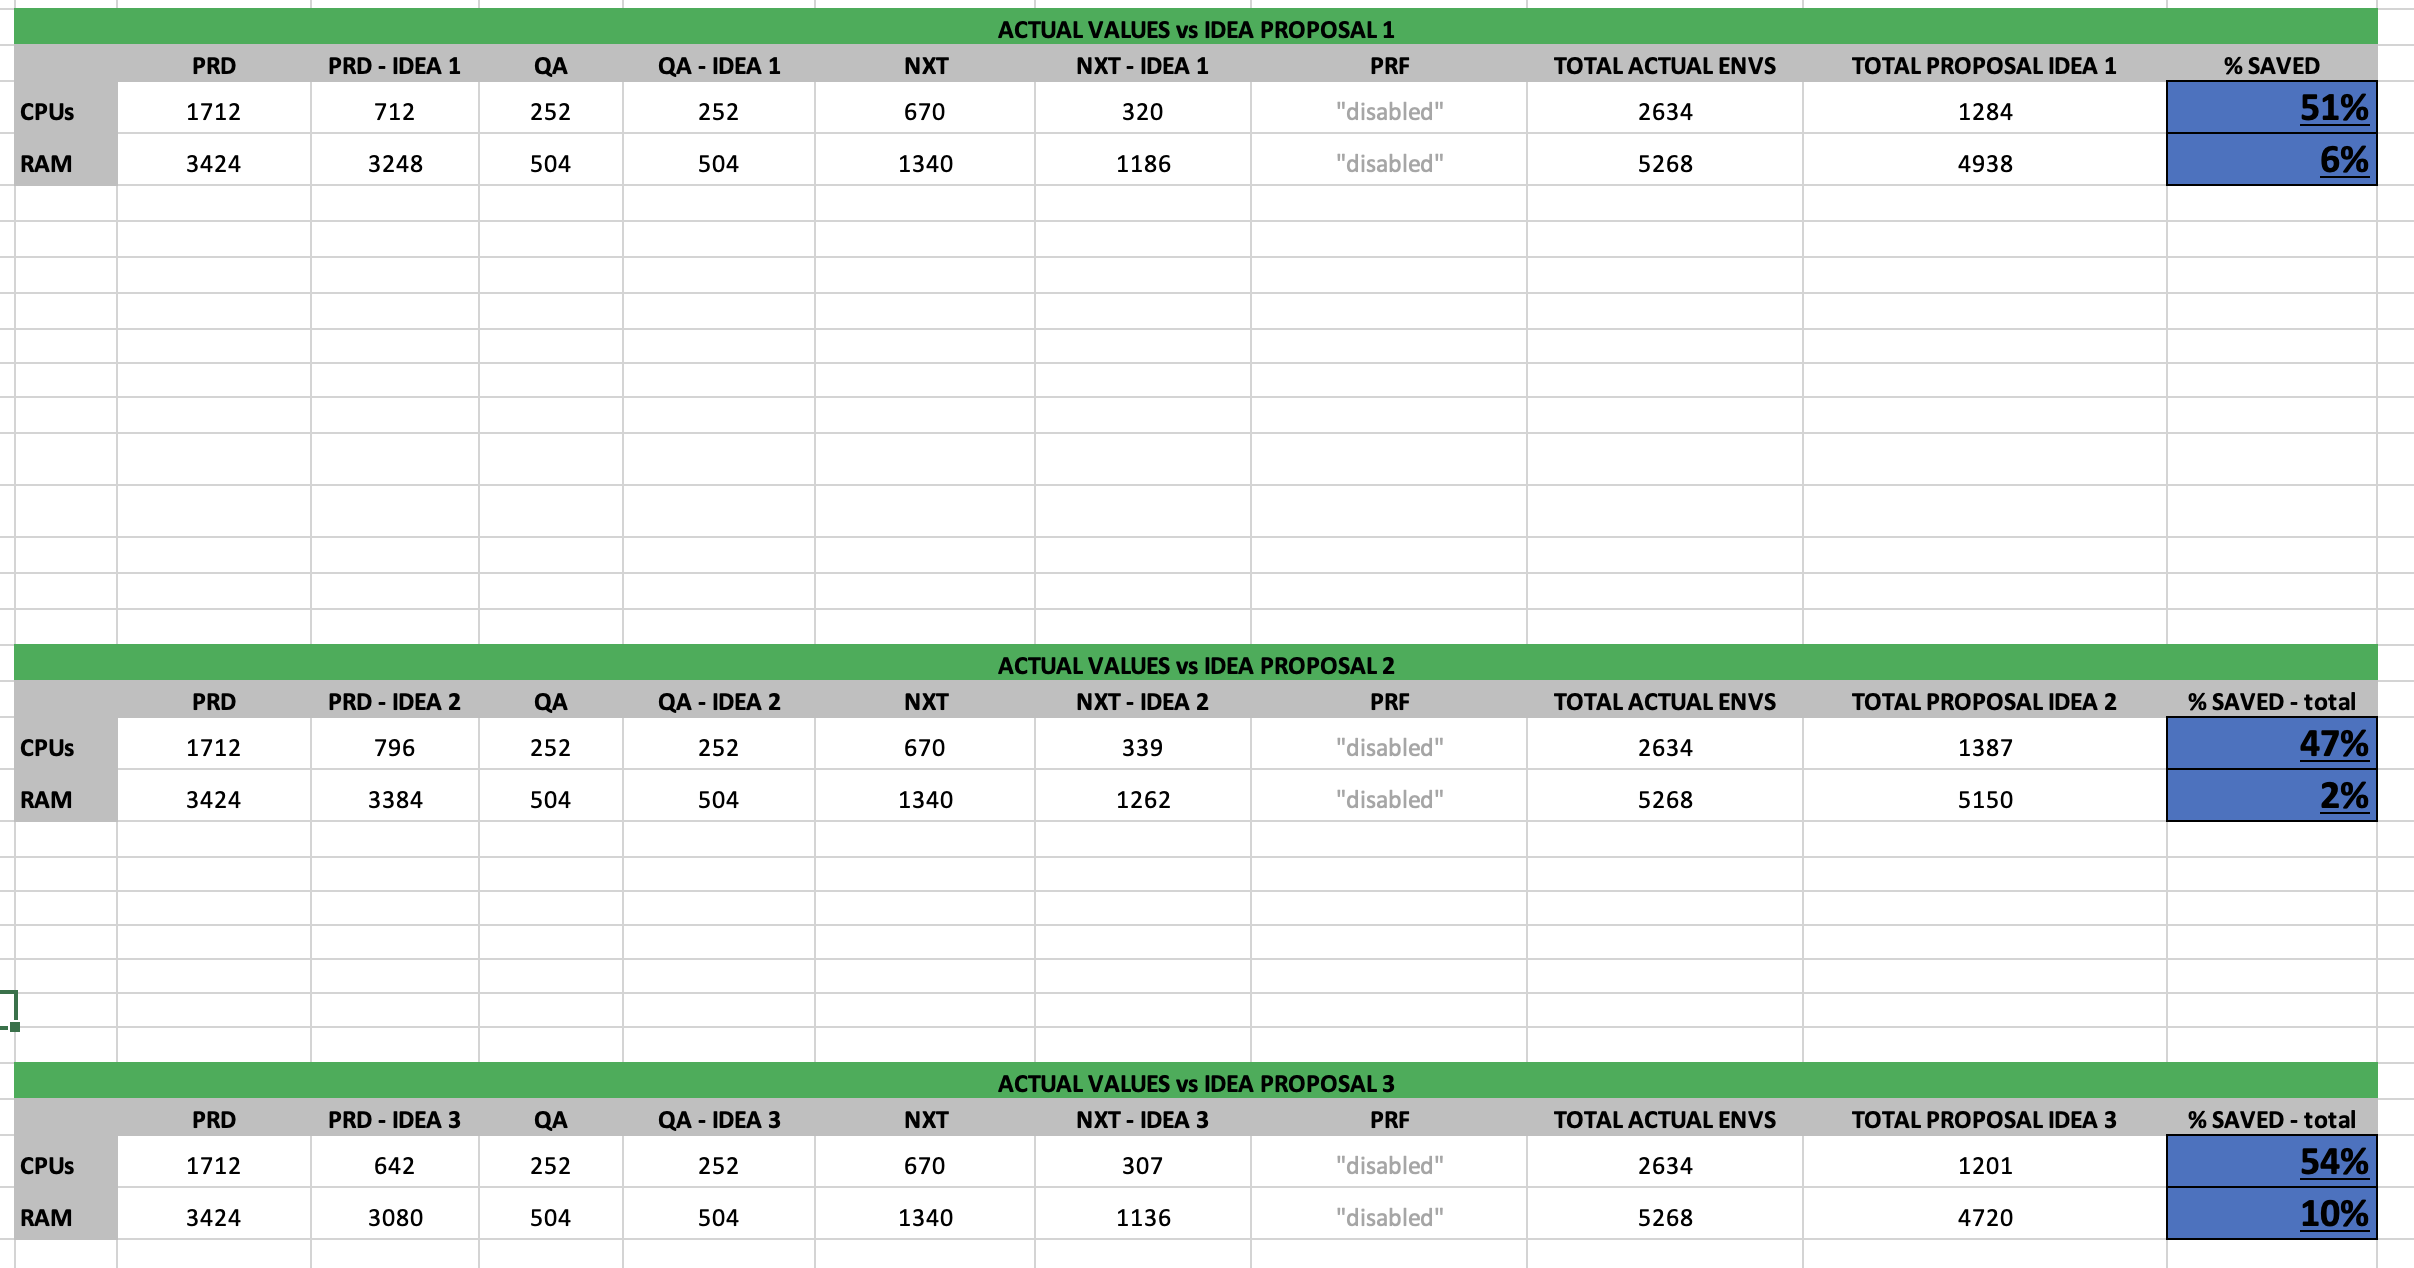
\includegraphics[scale=0.4]{media/content/analise/proposal-comparison.png}}
  \caption{Comparação de propostas de atualização}
  \label{comparison-proposal}
\end{figure}

\subsection{Processo de implantação}

Após decidir qual a abordagem a ser seguida é necessário definir o processo de implantação a ser
seguido. Este processo deve ser claro e conciso de forma a garantir que todas as equipas envolvidas
compreendam o processo que vai ser implementado e, desta forma, maximizar a probabilidade de
sucesso da intervenção. 

Este processo foi dividido em três passos que vão ser descritos e analisados de seguida. Por uma
questão de simplicidade no trabalho de análise, todos os quadros apresentados de seguida têm por 
base apenas os valores de recursos dos ambientes de produção, ou seja, para obter os valores reais
de redução de recursos deve ser necessário ainda ter em conta os recursos dos restantes ambientes
e multiplicar todos os resultados por dois já que todas as alterações devem ser replicadas em 
ambos os \glspl{dc}. Esta simplificação foi feita já que todas estas variáveis adicionais podem 
ser desprezadas dadas as semelhanças entre ambientes e a dimensão total da infraestrutura em
análise.

Como analisado anteriormente, a Figura \ref{strat-current} representa o estado atual dos 
\glspl{cluster}. Este é o ponto de partida para esta intervenção. 

No primeiro passo, representado na Figura \ref{strat-1}, é efetuada uma redução de recursos 
de ambos os \glspl{cluster}. Esta redução parte do princípio de que, sendo possível aplicar a 
solução final apresentada anteriormente, então, por definição, as topologias devem ser capazes de
operar sem problemas usando estes novos \glspl{flavour}. Esta intervenção só por si, representa
46\% de redução no uso total de \ac{CPU} (no ambiente de produção).

\begin{figure}[H]
  \centerline{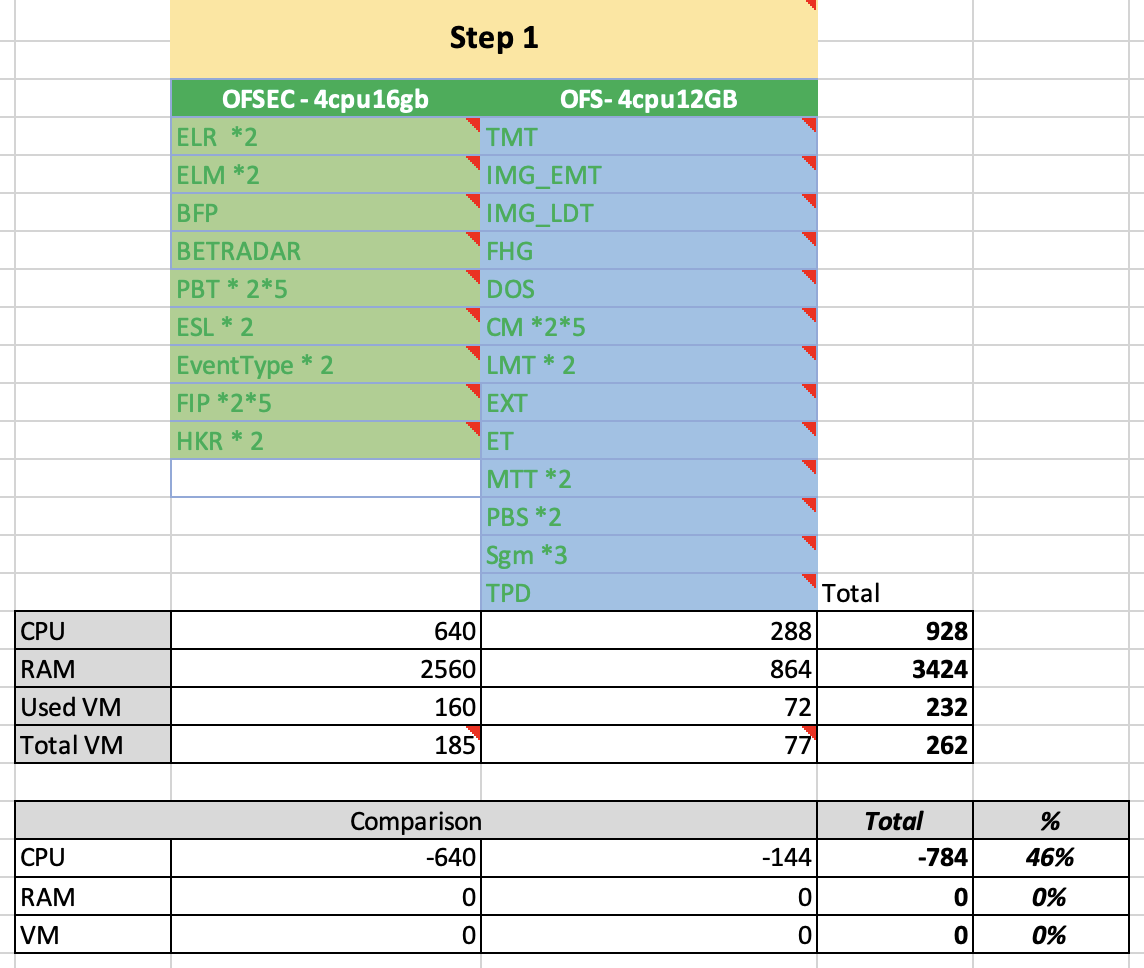
\includegraphics[scale=0.5]{media/content/analise/strat-1.png}}
  \caption{Processo de implantação - Passo 1}
  \label{strat-1}
\end{figure}

O segundo passo foi dividido em duas etapas - a criação do novo \gls{cluster}, representado na 
Figura \ref{strat-2} e a migração das topologias entre \glspl{cluster} (Figura \ref{strat-2_1}).

\begin{figure}[H]
  \centerline{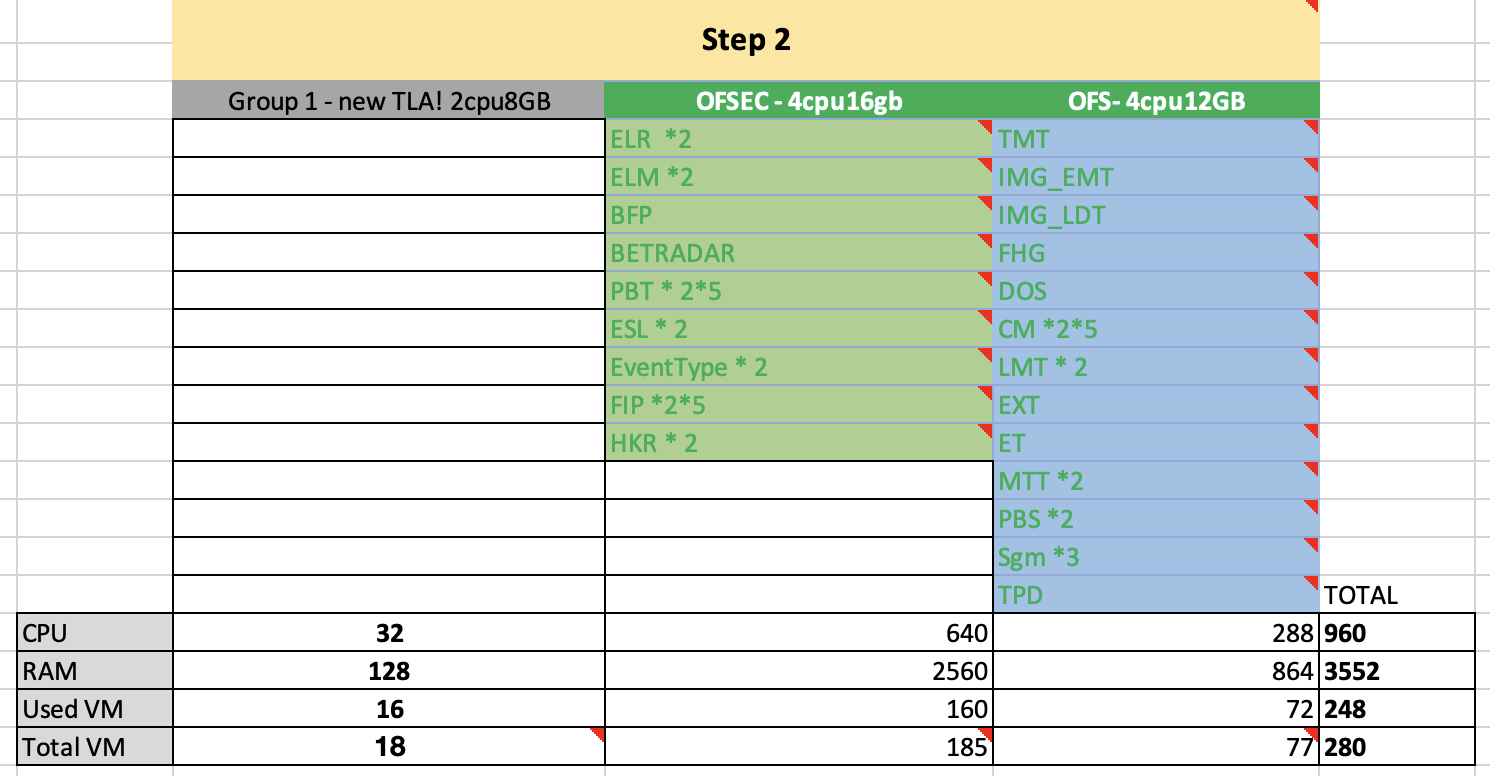
\includegraphics[scale=0.5]{media/content/analise/strat-2.png}}
  \caption{Processo de implantação - Passo 2}
  \label{strat-2}
\end{figure}

A segunda etapa deste passo é a etapa mais crítica de todo o processo, isto porque, nesta fase, é
crucial ter a total compreensão dos processos de replicação e \gls{failover} de cada topologia de
forma a minimizar o tempo de indisponibilidade de cada serviço.

\begin{figure}[H]
  \centerline{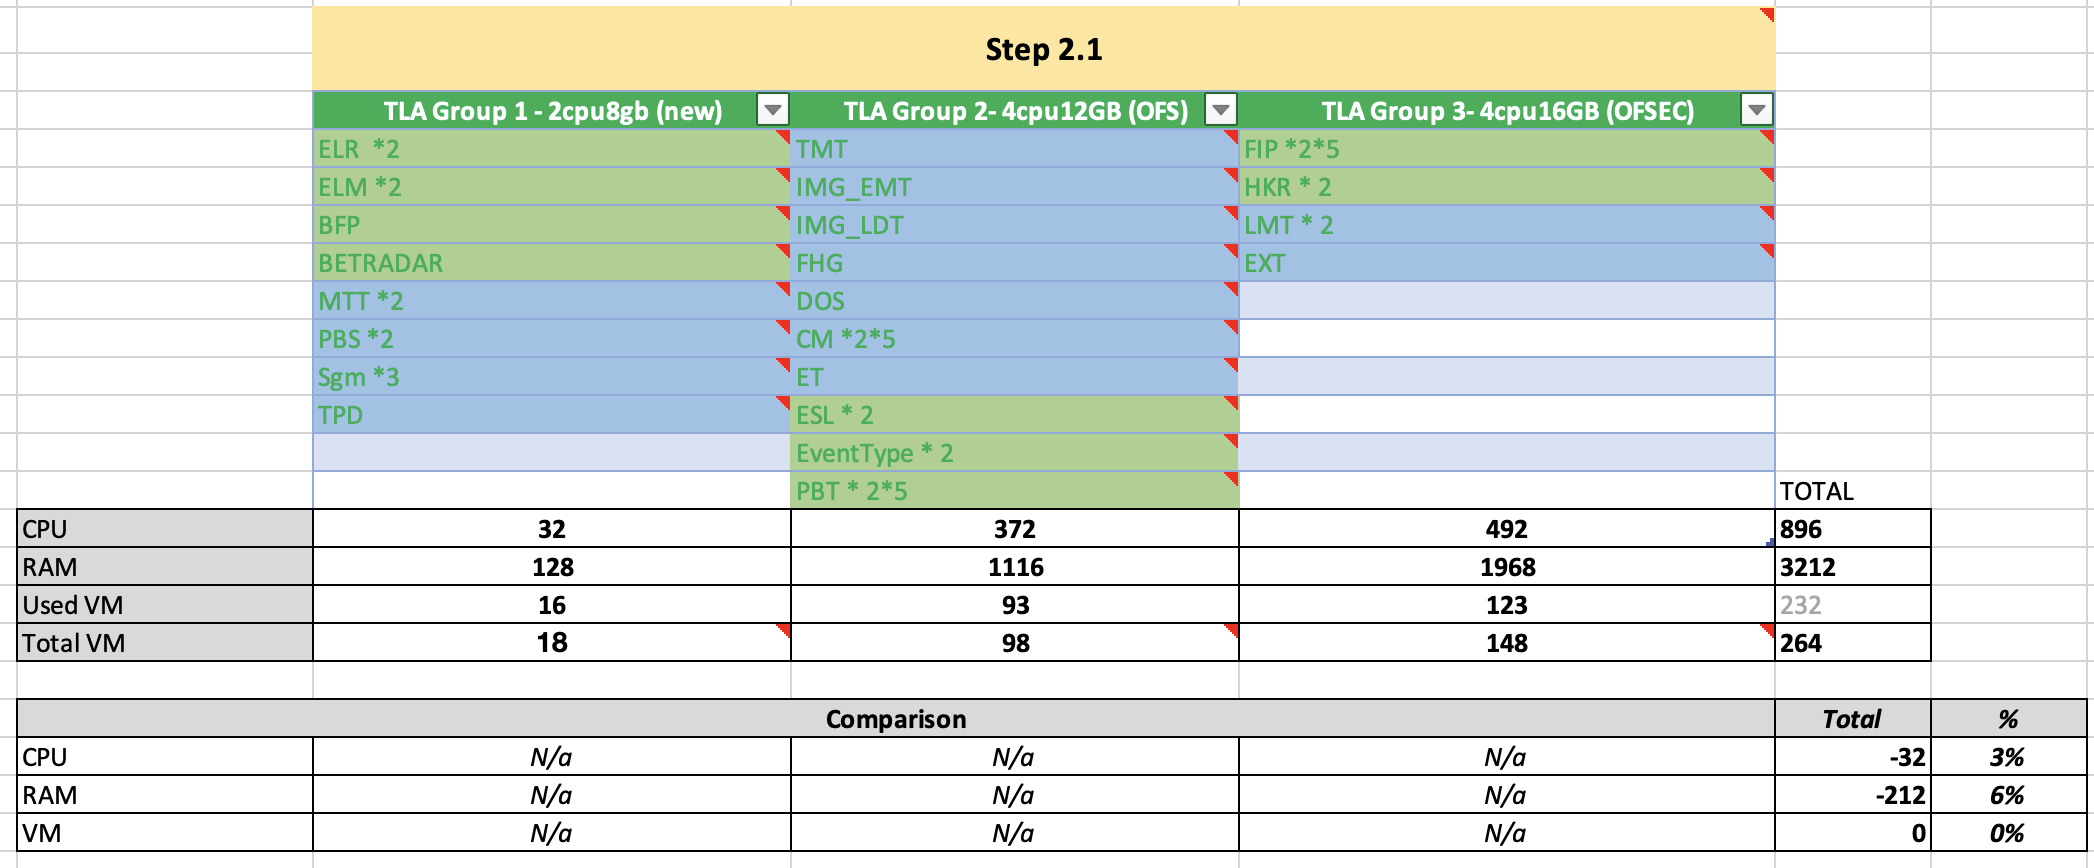
\includegraphics[scale=0.4]{media/content/analise/strat-2_1.png}}
  \caption{Processo de implantação - Passo 2.1}
  \label{strat-2_1}
\end{figure}

O terceiro, e último, passo, representando na Figura \ref{strat-3}, representa uma nova redução 
do \gls{flavour} de um dos \glspl{cluster}. Este passo é em todo semelhante ao primeiro, mas é
apenas necessário efetuar esta redução no segundo \gls{cluster}.

\begin{figure}[H]
  \centerline{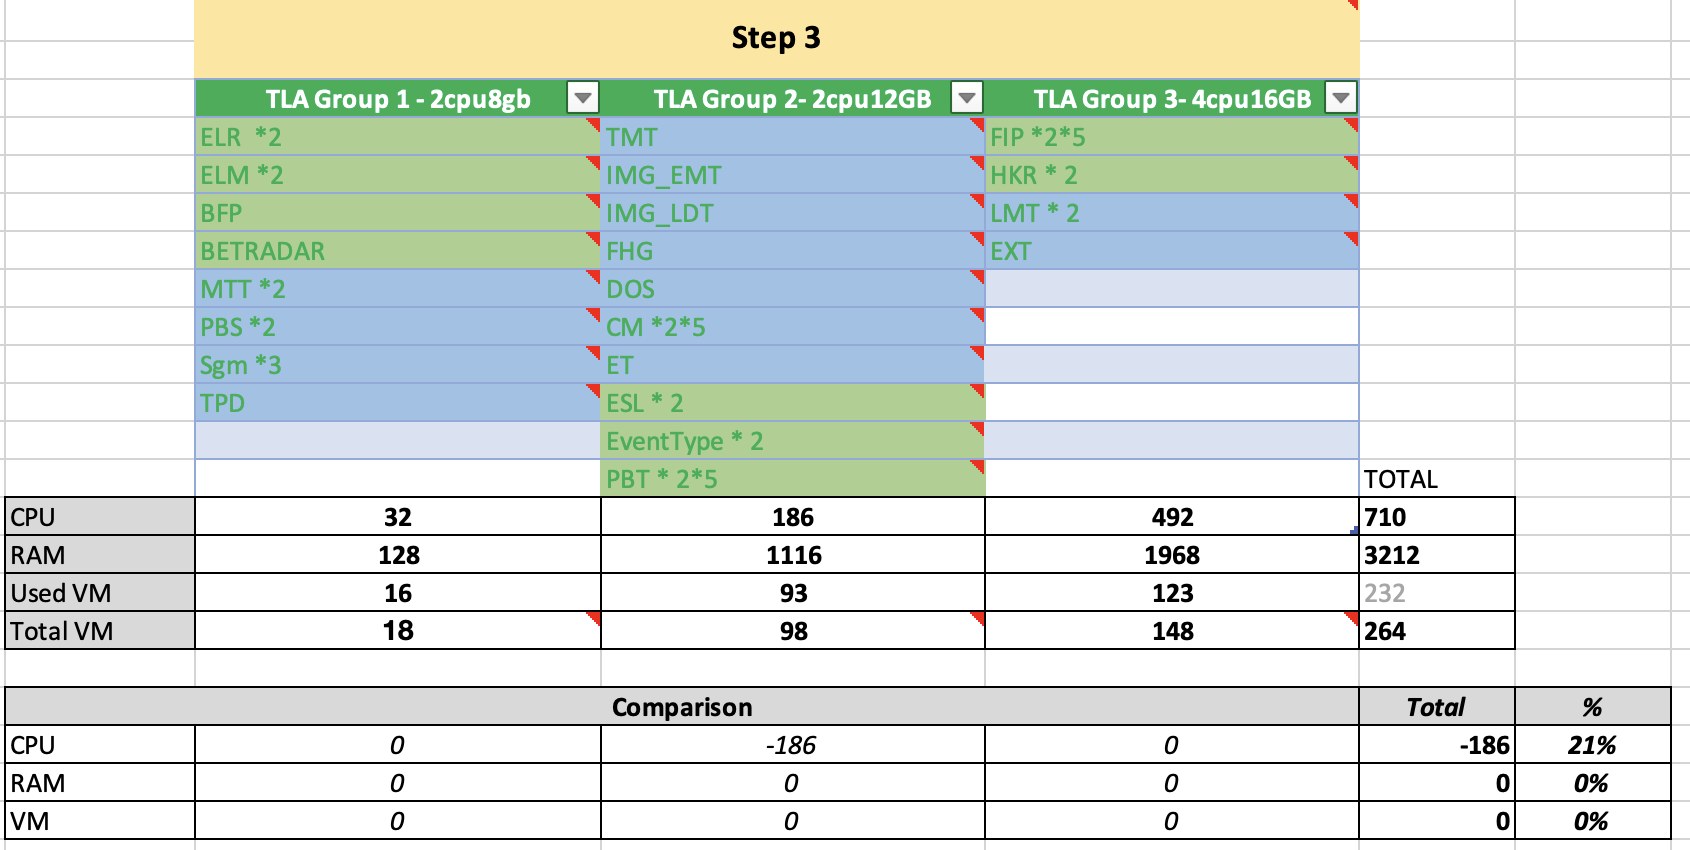
\includegraphics[scale=0.5]{media/content/analise/strat-3.png}}
  \caption{Processo de implantação - Passo 3}
  \label{strat-3}
\end{figure}

Após todo este processo a estrutura em que estão hospedadas as topologias encontra-se na forma
otimizada proposta anteriormente. Este processo sofre pequenas alterações entre ambientes já que 
os \glspl{flavour} não são iguais entre estes. Além disso, durante este processo tiveram que ser 
analisadas outras questões igualmente relevantes para garantir que esta migração era possível como 
é o caso da capacidade de comunicação do \textit{Zookeeper}.

O \textit{Zookeeper} é utilizado por todos estes \glspl{cluster} para garantir a resiliência das 
topologias e, por consequência, poderia não ter a capacidade de comunicar com um \gls{cluster}
adicional. Após analisar esta questão com as equipas responsáveis pela infraestrutura foi 
determinado que esta questão representava um problema crítico para o desempenho do 
\textit{Zookeeper}, logo, a proposta foi aprovada.


\oddPageStart
\chapter{Implementação da Solução}
\label{sec:4-Implementacao}

Este capítulo aprofunda o processo de desenvolvimento da solução para o problema do projeto em 
análise de acordo com a análise e os princípios de \textit{design} discutidos no capítulo anterior. 
Além disso, é efetuada uma análise cuidada dos resultados obtidos através das decisões anteriores, 
revelando os resultados consequentes e a sua concordância com os objetivos discutidos anteriormente.

\section{Tecnologias Utilizadas}

Durante o desenvolvimento do projeto, foram utilizadas várias tecnologias e ferramentas para a 
implementação da solução. Entre as mais relevantes, destacam-se:

\begin{itemize}
  \item \textbf{Apache Storm \cite{storm}:} \textit{Framework} de processamento de 
    \textit{streaming} em tempo real;
  \item \textbf{Apache Kafka \cite{kafka}:} Plataforma de mensagens distribuída;
  \item \textbf{Apache Zookeeper \cite{zookeeper}:} Serviço de coordenação distribuída;
  \item \textbf{Grafana \cite{grafana}:} Plataforma de análise e visualização de dados;
  \item \textbf{Nimbus \cite{nimbus}:} Servidor centralizado que coordena e distribui as topologias 
    do \textit{Apache Storm};
  \item \textbf{Splunk \cite{splunk}:} Plataforma de análise de eventos e dados;
\end{itemize}

\section{Descrição da implementação}

\todo[inline]{TODO}

\todo[inline]{Incluir BPMNs dos processos de pipelines para alterações de flavours + rollback}

\todo[inline]{Incluir BPMNs do processo de criação de novos clusters (simplificado}

\section{Testes}

\todo[inline]{TODO}

\section{Avaliação da Solução}

\todo[inline]{TODO}


\oddPageStart
\chapter{Conclusões}
\label{sec:5-Conclusoes}

Este capítulo final, apresenta uma síntese dos pontos mais relevantes do trabalho
desenvolvido. Em primeiro lugar, é realizada uma validação dos objetivos inicialmente propostos. 
De seguida, são tecidas as limitações e o trabalho futuro, visto que nenhum projeto está isento de 
barreiras. Na secção final, é realizada uma apreciação crítica, com o intuito de salientar pontos
positivos e menos positivos no decorrer do projeto.

\section{Objetivos concretizados}

Conforme é possível verificar nos capítulos \nameref{sec:2-EstadoArte}, \nameref{sec:3-Analise} 
e \nameref{sec:4-Implementacao} todos os objetivos traçados na subsecção \nameref{sec:1-obj} 
foram atingidos na sua totalidade. A Tabela \ref{tab:obj} mostra que todos os objetivos 
foram completamente realizados.

\begin{table}[H]
  \begin{center}
    \caption{Visão geral dos objetivos técnicos alcançados}
    \vspace{2mm}
    \label{tab:obj}
    \begin{tabular}{|l|c|}
      \hline
      \textbf{Objetivo} &
      \multicolumn{1}{l|}{\textbf{Grau de realização}} \\ \hline
      \begin{tabular}[c]{@{}l@{}}xxx\end{tabular} &
      100\% \\ \hline
    \end{tabular}
  \end{center}
\end{table}

\section{Limitações e trabalho futuro}



\section{Apreciação final}



% Referências
\newpage
\bibliographystyle{unsrt}
\nocite{*}\bibliography{ref.bib}

\begin{appendices}
  \chapter{Anexo A} 	
\label{appendix-a}

\begin{figure}[H]
  \centerline{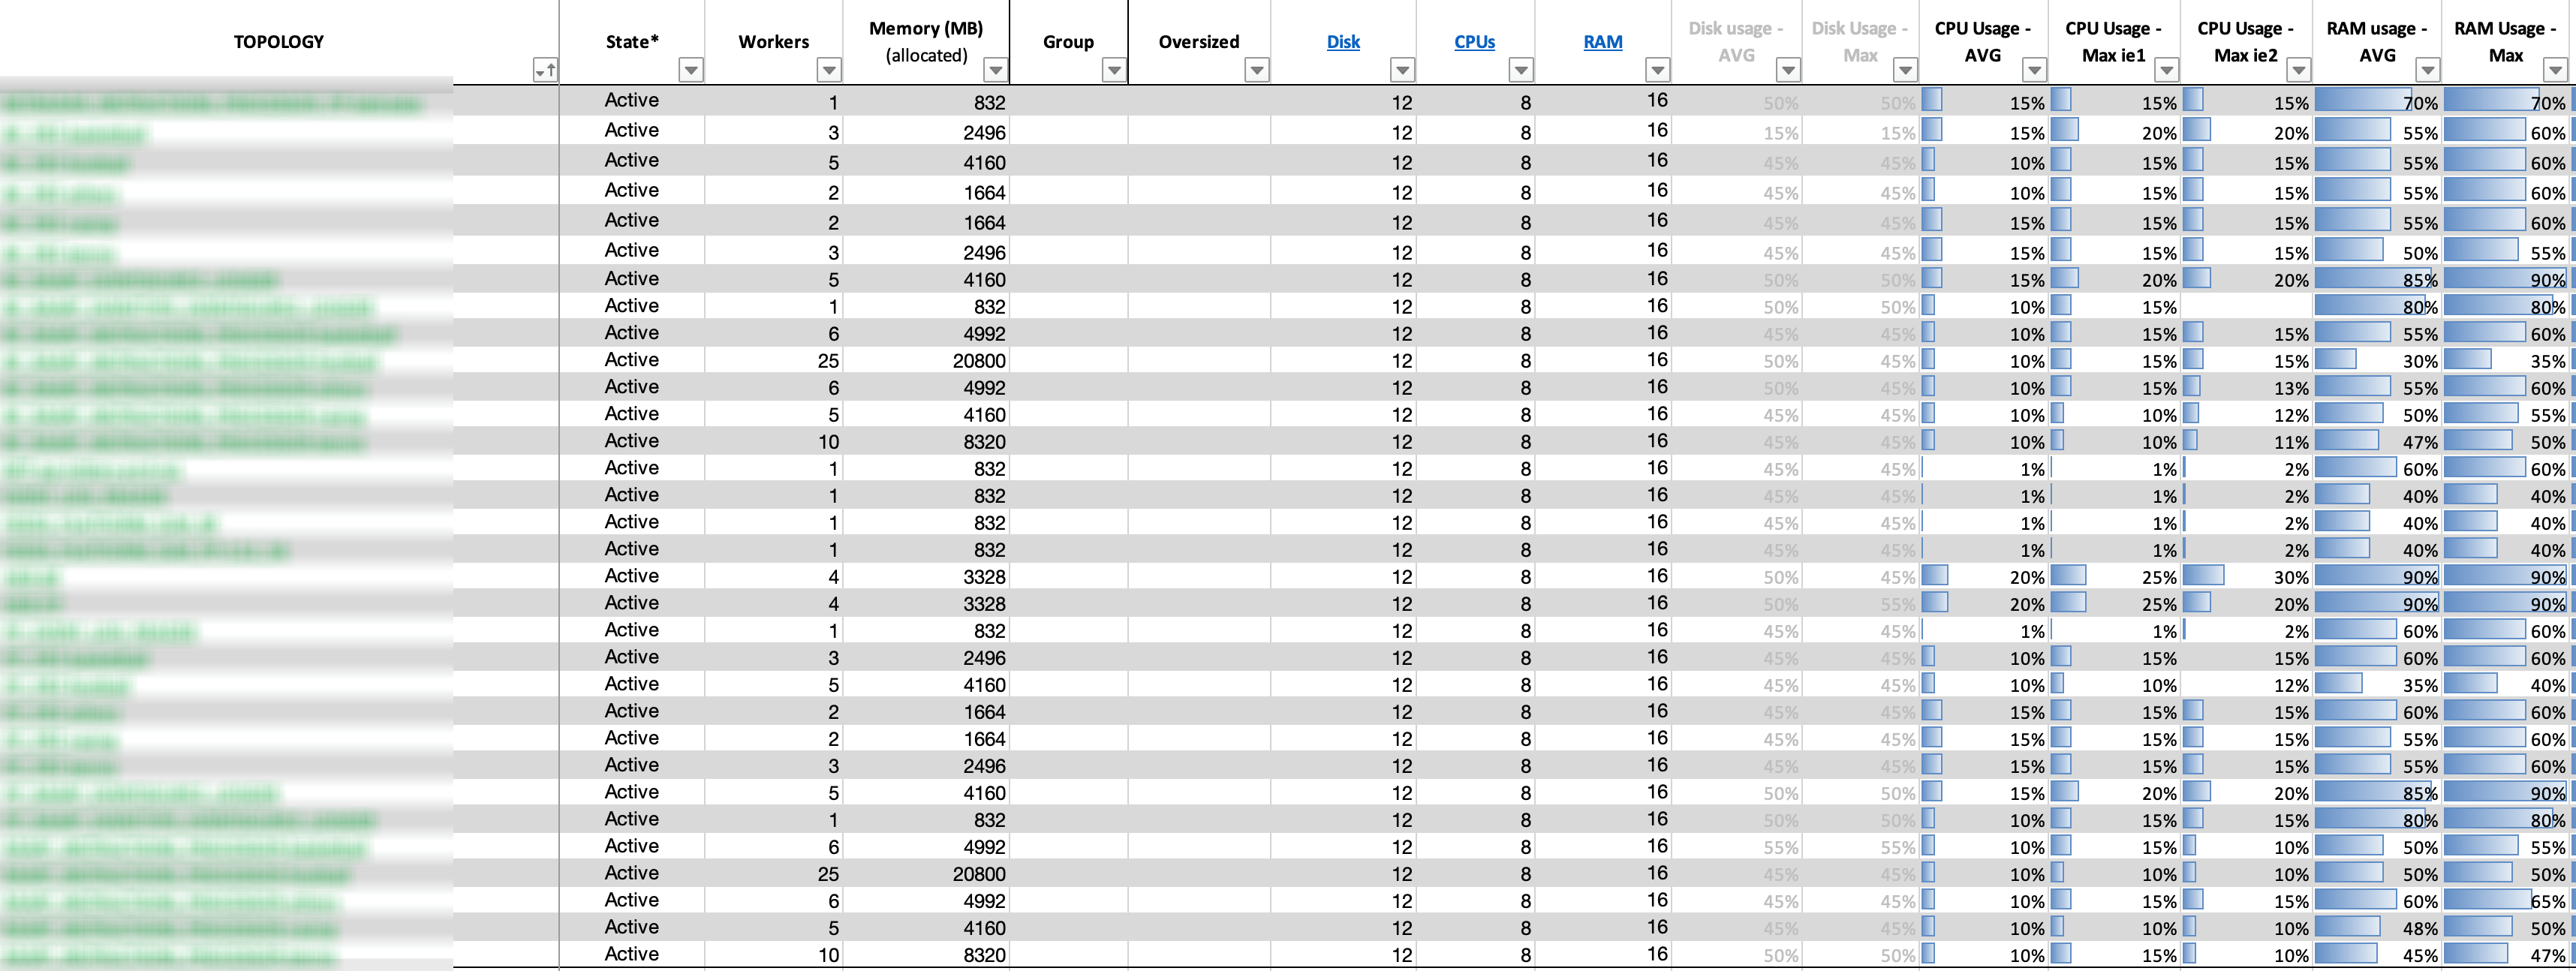
\includegraphics[scale=0.3]{media/content/analise/analise-ofsec-1.png}}
  \caption{Análise do uso de recursos de um dos \textit{clusters} - Parte 1}
  \label{analise-ofsec-1}
\end{figure}

\begin{figure}[H]
  \centerline{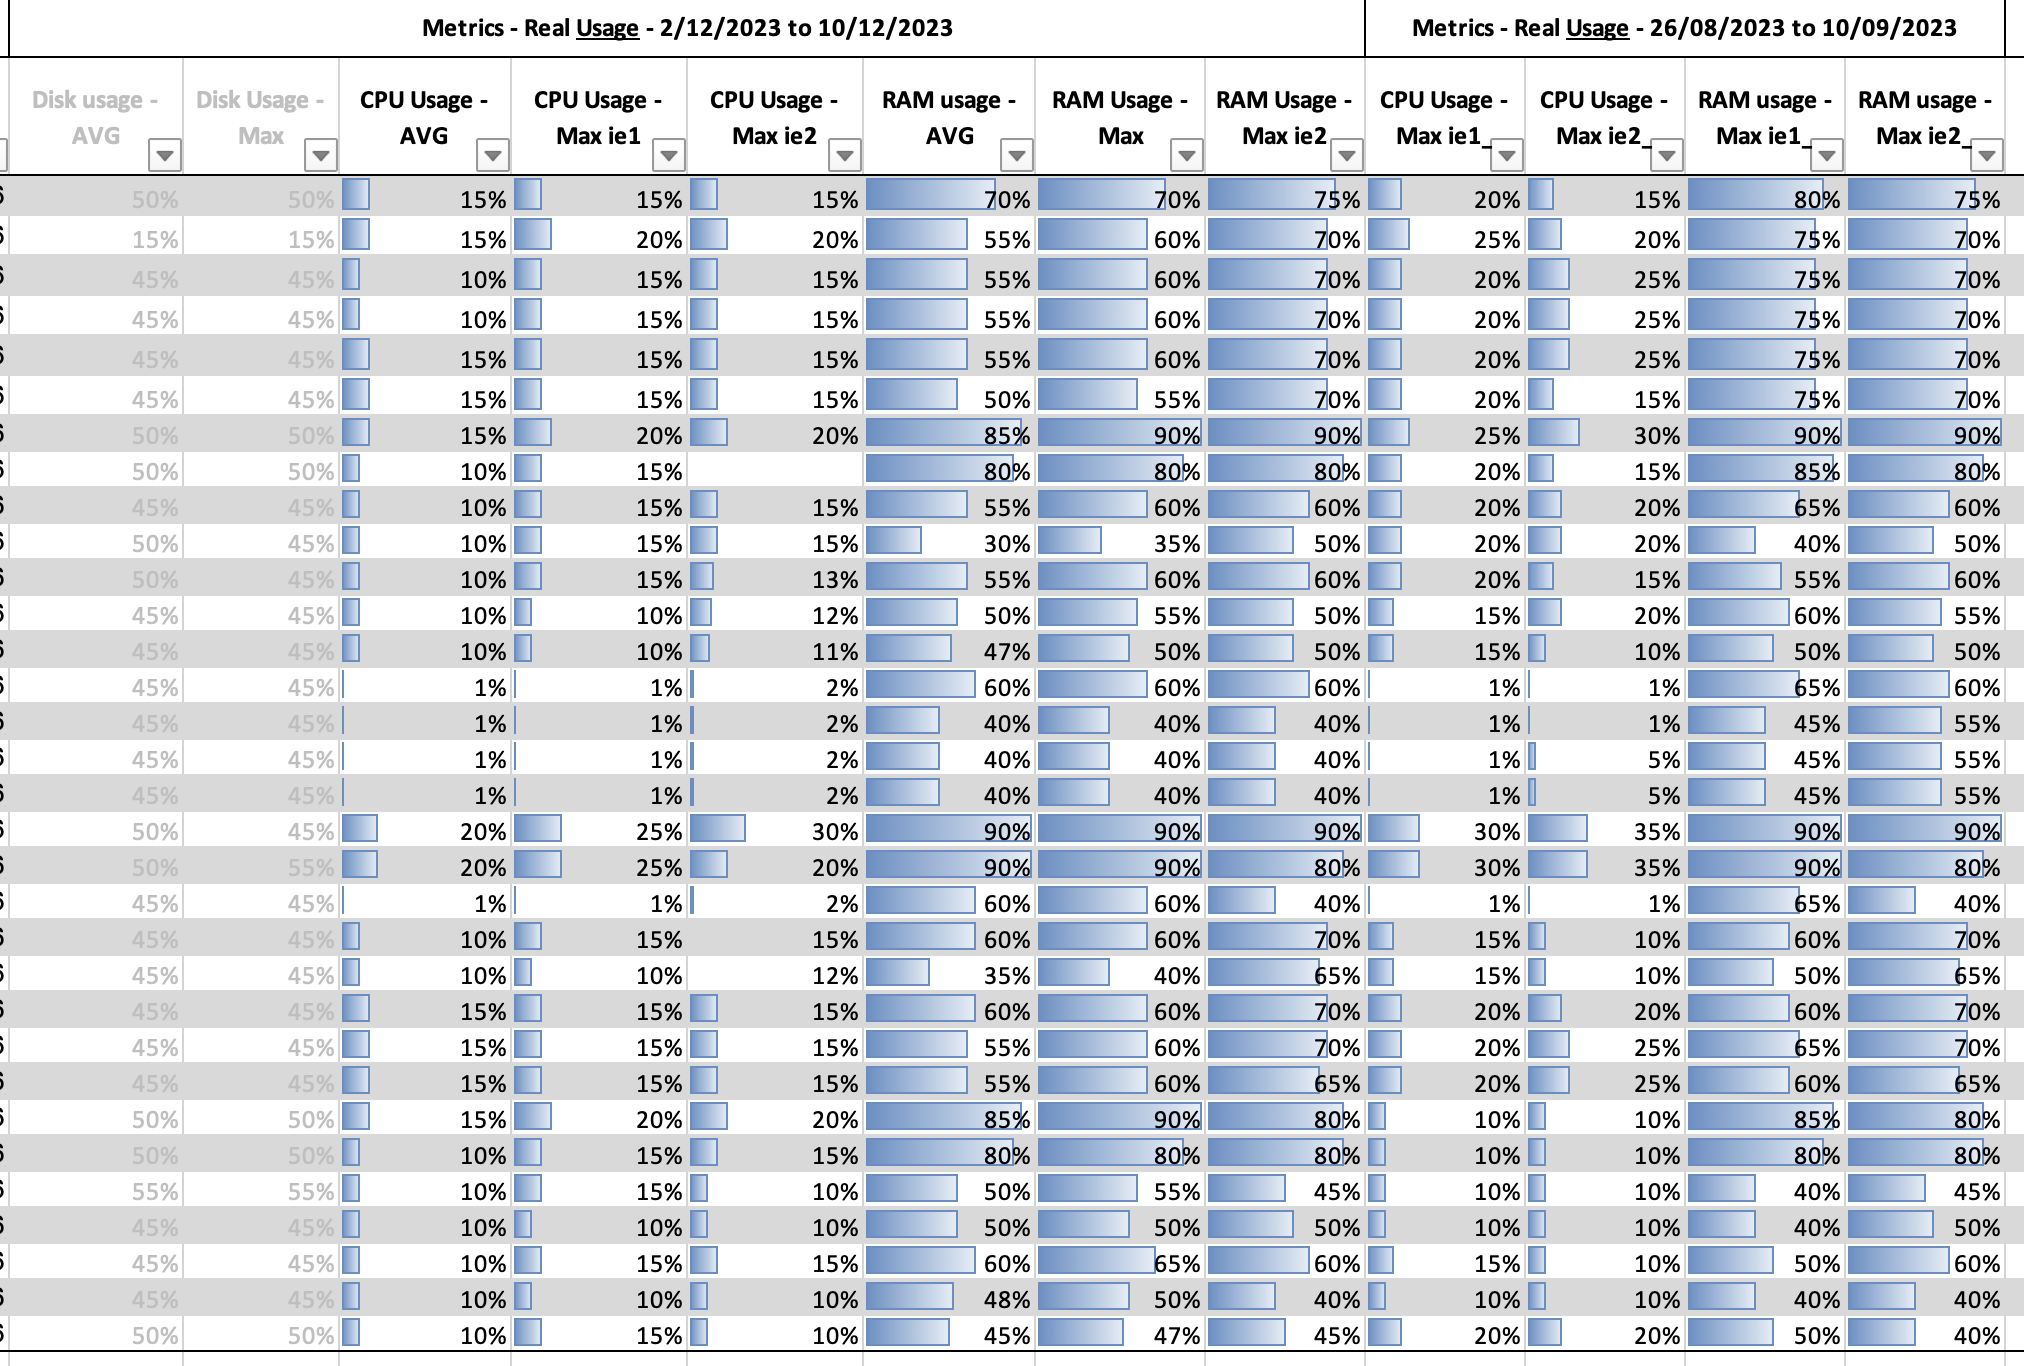
\includegraphics[scale=0.3]{media/content/analise/analise-ofsec-2.png}}
  \caption{Análise do uso de recursos de um dos \textit{clusters} - Parte 2}
  \label{analise-ofsec-2}
\end{figure}

\begin{figure}[H]
  \centerline{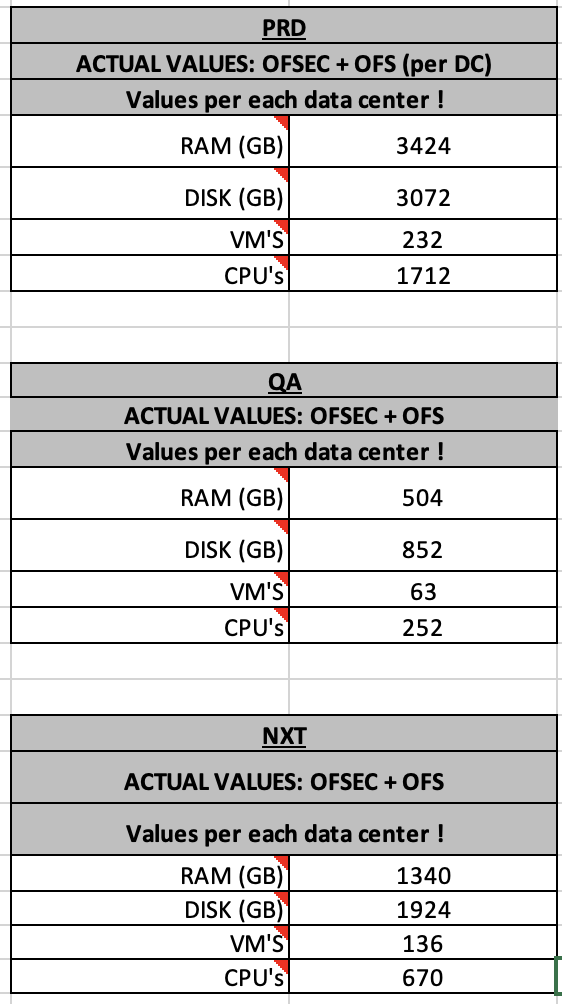
\includegraphics[scale=0.5]{media/content/analise/resources-per-env.png}}
  \caption{Uso de recursos por ambiente}
  \label{resource-usage}
\end{figure}

\begin{figure}[H]
  \centerline{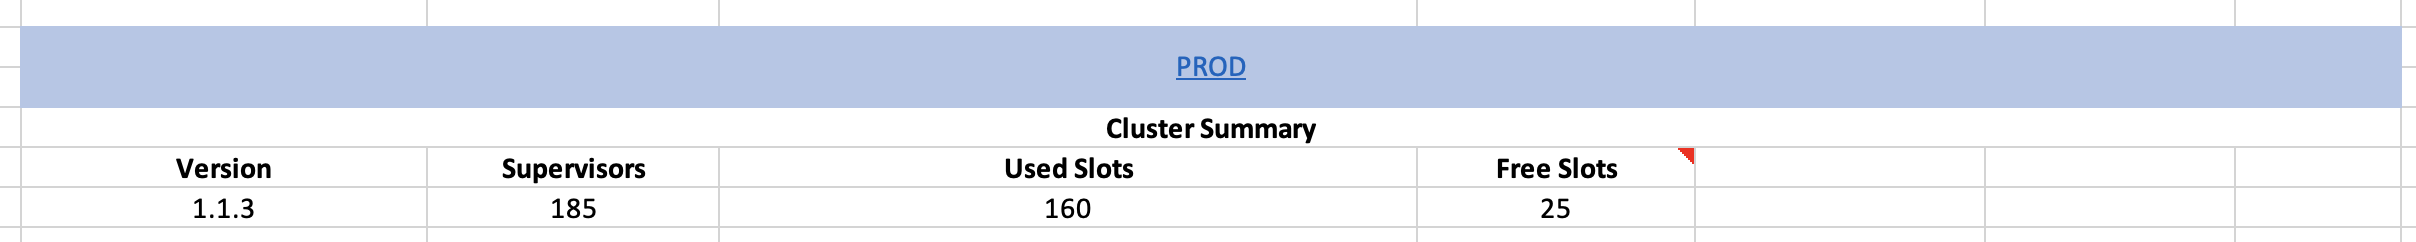
\includegraphics[scale=0.4]{media/content/analise/info-ofsec-prod.png}}
  \caption{Informação de número de VMs de um dos \textit{clusters} em produção}
  \label{vms-info}
\end{figure}


  \include{appendices/B-Appendix}
\end{appendices}

\end{document}
